\documentclass[pdftex,twocolumn,epjc3]{svjour3} 
\RequirePackage[T1]{fontenc}
\smartqed  % flush right qed marks, e.g. at end of proof
\RequirePackage{graphicx}
\RequirePackage{mathptmx}      % use Times fonts if available on your TeX system
\RequirePackage{flushend}
\RequirePackage[numbers,sort&compress]{natbib}
\RequirePackage[colorlinks,citecolor=blue,urlcolor=blue,linkcolor=blue]{hyperref}

\journalname{Eur. Phys. J. C}


\usepackage{amsmath,amssymb,amsfonts}
\usepackage{algorithmic}
\usepackage{graphicx}
\usepackage{textcomp}
\usepackage{float}
\usepackage{etoolbox}

\usepackage{url}
\usepackage{listings}
\usepackage{pdfpages}
\usepackage[english]{babel}
\usepackage{xcolor,colortbl}
\usepackage{scalerel}
\newcommand{\customer}{customer}
\renewcommand{\sp}{SP}

\newcommand{\normal}{n}
\newcommand{\dispute}{d}
\newcommand{\abnormal}{\overline{n}}
\newcommand{\abdispute}{\overline{d}}

\newcommand{\PoD}{$\mathrm{PoD}$}
\newcommand{\PoP}{$\mathrm{PoP}$}
\newcommand{\cid}{$\mathrm{cid}$}

\newcommand{\floor}[1]{\left\lfloor #1 \right\rfloor}
\newcommand{\ceil}[1]{\left\lceil #1 \right\rceil}

\newcommand{\plus}{+}
\newcommand{\minus}{-}
\newcommand\neutral[1][.75]{\mathbin{\ThisStyle{\vcenter{\hbox{%
  \scalebox{#1}{$\SavedStyle\bullet$}}}}}%
}

\def\SINGLECOLUMN{SINGLE}
\def\DOUBLECOLUMN{DOUBLE}
\def\JOURNALIEEE{IEEE}
\def\JOURNALELS{ELS}

\newcommand\TITLE{Anonymous provision of privacy-sensitive services using blockchain and decentralised storage}
\newcommand\STANLONG{Stanis\l{}aw Bara{\'n}ski}
\newcommand\JULLONG{Julian Szyma{\'n}ski}
\newcommand\HIGILONG{Higinio Mora}
\newcommand\STAN{S. Bara{\'n}ski}
\newcommand\JUL{J. Szyma{\'n}ski}
\newcommand\HIGI{H. Mora}

\newcommand\ABSTRACT{
Lawyers, laboratories, auditors or banks, in order to provide services, require data often containing sensitive personal information.

Examples of sensitive services are genetic tests, parenthood tests, STD tests, credit score computation or legal advice. 

The processing of personal data, especially when providing services involving sensitive data like health records, biological materials, or legal documents, exposes both users and service providers (SP) to privacy risks.

SPs are at risk of violating GDPR, CPAA, and other legal regulations, while customers are at risk of losing their privacy.

We observe that personal data is often only used for logistical purposes, such as payments or communication, and could be provided anonymously if such methods were available.

In this work, we propose a solution that allows the provision of services without the collection of personal data. We use anonymous payment methods such as cash and anonymous cryptocurrencies, blockchain technology to achieve fairness, and distributed content-addressable storage networks to deliver results.

Compared to other solutions, our protocol achieves anonymity with weaker assumptions, supports physical materials and conflict resolution, and in conflict-free transactions does not require the customer to interact with the blockchain, demonstrating better practicality.

In this work, we analyse the fairness of our protocol and implement it using Ethereum technology as a message board, Monero as an anonymous payment method, and Powergate (IPFS and Filecoin) as a decentralised storage network.
}


\newcommand\ACKNOWLEDGEMENTS{
The work has been supported partially by the founds of Department of Computer Architecture Faculty of Electronics, Telecommunications and Informatics, Gdańsk University of Technology.
}

\newcommand\LASTVISITED{(last visited Jan. 31, 2023)}

\begin{document}

\title{\TITLE}

\author{\STANLONG\thanksref{e1,addr1}
        \and \JULLONG{}\thanksref{e2,addr1}
        \and \HIGILONG{}\thanksref{e3,addr2}
}


\thankstext{e1}{e-mail: stanislaw.baranski@pg.edu.pl}
\thankstext{e2}{e-mail: julian.szymanski@pg.edu.pl}
\thankstext{e3}{e-mail: hmora@ua.es}

\institute{Department of Electronic, Telecommunication and Informatics, Gdansk University of Technology, Narutowicza 11/12 80-233 Gdansk Poland\label{addr1}
          \and
          Department of Computer Science Technology and Computation, University of Alicante, San Vicente del Raspeig, 03690 Alicante Spain \label{addr2}
}


\date{Received: date / Accepted: date}
% The correct dates will be entered by the editor

\maketitle

\begin{abstract}
  \ABSTRACT{}
  
  \newcommand{\sep}{ \and }
  \keywords{Anonymity\sep{} blockchain\sep{} diagnosis\sep{} e-commerce\sep{} fair-exchange\sep{} privacy\sep{} services}
\end{abstract}

\section{Introduction}
\label{sec:introduction}
Diagnostic services such as paternity tests, doping tests or venereal disease tests are carried out in diagnostic centres that require clients to provide biological material such as blood, urine, stool or saliva. Unfortunately, clients are often forced to reveal their identity in order to complete transactions. Such a combination of personal information with biological materials exposes clients to significant privacy risks.

Other examples of sensitive services include anonymous complaints or legal services, such as legal advice, which may require disclosure of financial transaction history and confidential legal documents. Banking services, such as credit scoring, may require sensitive personal information, such as medical records and financial transaction history.

Providing personal information exposes users to privacy risks, i.e. the potential loss of control over personal information \cite{smithInformationPrivacyResearch2011}.

Such personal information can be used deliberately or by accident (e.g. theft) for insider disclosure, unauthorised access or commercial gain. For example, by reselling it to marketers, financial institutions, other businesses, government agencies or even cybercriminals. 
This, in turn, can lead to unintentional GDPR or CCPA breaches, profiled advertising, or even criminal activity such as identity theft or illegal tracking and surveillance~\cite{smithInformationPrivacyResearch2011}.

Public figures such as influencers, politicians or celebrities are particularly vulnerable to this type of attack, as exposure of their health records, purchasing habits or legal documents can threaten their reputation, position or be used for blackmail.

The problem is compounded when personal information is linked to health records, legal documents or biological materials such as DNA, saliva or blood.
In such situations, clients may be reluctant to provide their personal information to the SP and therefore withdraw from the service. Both parties are harmed as the client does not receive a diagnosis relevant to their health and the SP loses potential clients.

The guarantee of privacy of personal data is often based solely on trust in the SP's staff and the security of their IT systems. However, we observe that personal data is often used only for logistical purposes, such as payment or communication, and could be provided anonymously if such methods were available.

It would be desirable for customers to keep their identity private while still receiving the service. This could lead to a reduction in the trust that customers need to place in SPs and a reduction in the responsibility that SPs bear.

Examples of services that would benefit from the anonymity property are:
\begin{itemize}
    \item Patients who are willing to take a test, e.g. for drugs, STDs, paternity or steroids, have a strong incentive to keep the whole process private. The mere fact that they have taken the test—without revealing the result—is suggestive enough to be used as a premise in the event of a conflict.

    Currently, they have to take the risk that their personal data, materials and results will be stored securely and kept secret from any unauthorised actor (both curious employees and malicious attackers).


\item Individuals engaged in entrepreneurial activities may want to assess the risks and possible consequences of their actions.

By revealing their identity, they trust that the lawyer will not use this information for harmful actions.
\end{itemize}

Using Solove's Taxonomy of Privacy~\cite{soloveTaxonomyPrivacy2006}, our protocol aims to prevent the following privacy risks:
\begin{itemize}
    \item \textbf{Breach of confidentiality}, breaking a promise to keep an individual's information confidential;
    \item \textbf{Disclosure}, revealing true information about a person that affects the way others judge their character;
    \item \textbf{Identification}, linking information to a specific individual;
    \item \textbf{Secondary use}, using personal information for a purpose other than that for which they were collected.
\end{itemize}

We consider the following adversaries:
\begin{itemize}
    \item \textbf{Malicious insiders}: Individuals or entities with authorised access to the protocol's systems or data who may abuse their privileges to compromise customer privacy. This could include employees, contractors or service providers;
    \item \textbf{Government agencies}: Depending on the jurisdiction and the nature of the protocol, government agencies may have legal powers or national security interests that could affect customer privacy. For example, the potential for surveillance, data requests or legal intervention;
    \item \textbf{Malicious third-party services}: If the protocol relies on third party services or APIs, the privacy of customer data could be at risk if these services have inadequate security measures in place or if they engage in data sharing or tracking without the consent of the customer;
    \item \textbf{Hackers and cybercriminals}: Individuals or organised groups with malicious intent who may exploit vulnerabilities in the protocol's implementation, infrastructure, or supporting systems to gain unauthorised access to customer information.
\end{itemize}

In this work we explore the possibilities of anonymous service provision and propose a protocol that preserves customer privacy even in the event of a successful attack. Under realistic operational assumptions, we believe that decoupling personal information from materials, payment and communication achieves a sufficient level of anonymity.

However, a protocol that hides a customer's identity is difficult to secure and coordinate. In particular, conflicts between customers and service providers are difficult to resolve when there is no one to accuse.

We observe that the problem of anonymous service provision can be seen as a problem of fair exchange, where parties exchange some goods fairly, i.e. either both parties obtain the goods, or they both obtain nothing.

In our case, the customer who wants to use the service exchanges his materials and money with the SP for the result of the service.

Our review shows that none of the current systems is sufficient to achieve the desired goal. We propose an anonymous protocol for the provision of services that require physical materials. In the event of a dispute, either due to missed deadlines or incorrect results, the customer can disclose the entire interaction, prove the SP's misbehaviour to justice, and win the dispute.

To achieve this goal we use
\begin{itemize}
    \item \textbf{Blockchain}, to achieve fairness, i.e. as a means of proving that certain actions took place at a certain time without the Trusted Third Party (TTP).
    \item \textbf{Anonymous payment methods}, such as cash or anonymous cryptocurrencies, which allow customers to pay for services anonymously.
\item \textbf{Decentralised storage network} (e.g. IPFS) to provide results together with a provable storage network (e.g. Filecoin) to guarantee that the results are available to the customer even if the SP refuses to share the result.
    
    \item Cryptography:
    \begin{itemize}
        \item \textbf{Symmetric encryption}, to encrypt and decrypt the results published on the public networks.
        \item \textbf{Diffie-Helman key exchange (DHKE)}, to derive shared secrets for symmetric encryption.
        \item \textbf{Digital signatures}, to achieve authentication and non-repudiation of actions. 
    \end{itemize}
    
\end{itemize}

Figure~\ref{fig:protocol-overview} shows a simplified diagram of the protocol.

\begin{figure}[h!]
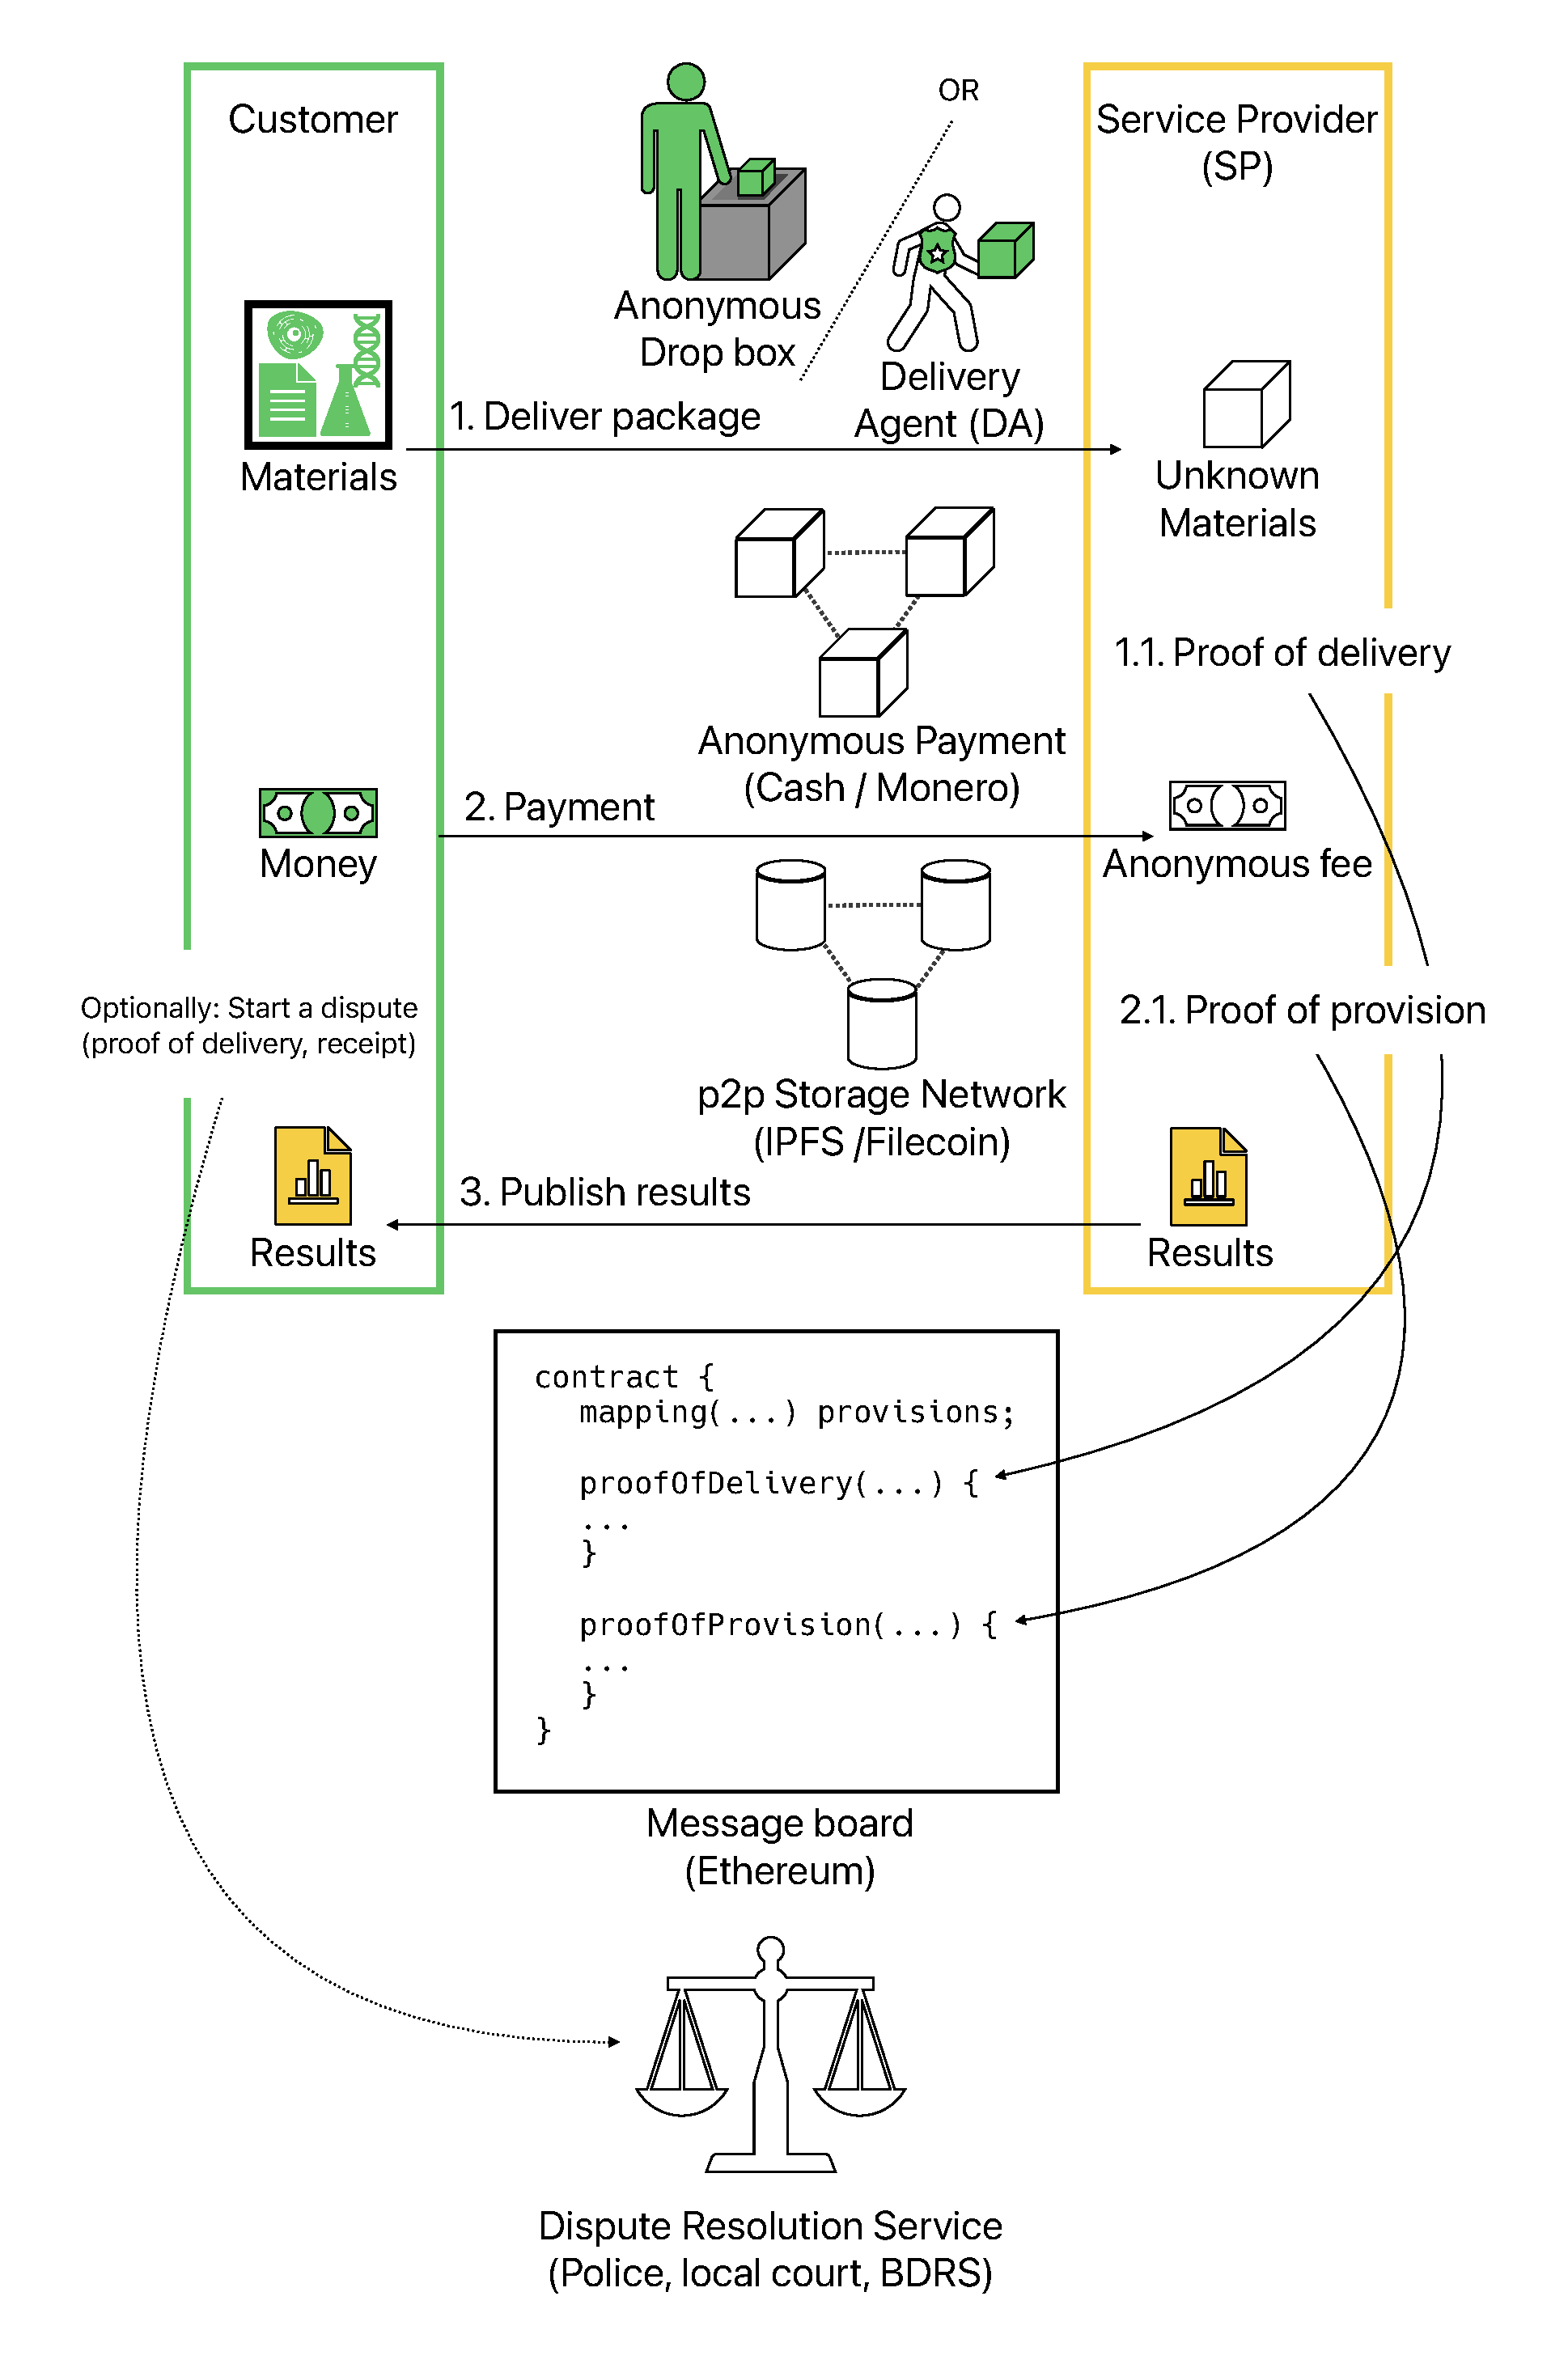
\includegraphics[width=\linewidth]{protocol-overview.pdf}
\centering
\caption{A simplified diagram of the protocol. The first step involves the delivery of the materials to the SP. The second step involves anonymous payment. The third step involves the delivery of the results to the customer. Each step is proven on the message board, protecting the fair party in a conflict situation.}

\label{fig:protocol-overview}
\end{figure}

\paragraph{}
The contribution of our paper is:
\begin{itemize}
\item we propose a protocol that upon a realistic operational and threat model:
  \begin{itemize}
  \item allows \textbf{anonymous} service provision involving \textbf{physical materials}, i.e., the service provider does not need to collect any personal information from the customer;
  \item achieves \textbf{fairness} by the use of blockchain and cryptographic proofs. We model the protocol as an interactive non-cooperative game and show fairness at each of its steps.
  \item \textbf{does not rely on a centralised TTP}, but uses a decentralised blockchain and a distributed content-addressable storage network;
  \item in conflict-free transactions does not require customers to interact with the blockchain, achieving better \textbf{user experience and practicality};
  \item guarantees the \textbf{remote availability of the results}, even in case of the SP denial of service.
  \end{itemize} 
\item We implement a working prototype of the protocol and provide open source code.
\item We systematise often misused definitions of anonymity, pseudonymity, linkability and traceability.
\item We propose a framework for analysing fairness in fair exchange protocols and use it to prove the fairness of our protocol.
\item We discuss possible improvements to the protocol using secure computation, self-sovereign identities, zero-knowledge proofs, and blockchain-based dispute resolution techniques.
\end{itemize}

Some authors have proposed blockchain-based fair exchange systems that could be adapted to service provision; however, to the best of our knowledge, we are the first to propose a system that satisfies all of the above properties. In particular, anonymity and physical delivery have rarely been addressed together, and if so, the protocol was based on TTP and impractical assumptions about the banking system~\cite{birjoveanuAnonymityFairexchangeEcommerce2015} or did not address the conflict between parties~\cite{altawyLelantosBlockchainBasedAnonymous2017}.


The rest of this paper is organised as follows.
In Section~\ref{sec:related-works} we review related works. 
Then in Section~\ref{sec:building-blocks} we discuss the building blocks of a dispute resolution system, blockchain as a message board, fairness, anonymous payments, storage network, availability of results and anonymity.
Section~\ref{sec:protocol} provides a detailed description of the protocol.
Section~\ref{sec:fairness-analysis} provides a fairness analysis of the proposed protocol.
Section~\ref{sec:experiments} presents the implementation of the protocol and the results of our experiments.
Section~\ref{sec:discussion} discusses possible improvements in terms of crowdsourced dispute resolution or dispute avoidance, self-sovereign identities (SSIs), anonymous delivery, and formal verification.
Finally, Section~\ref{sec:conclusion} concludes the paper.


\section{Related Works}\label{sec:related-works}
In this section, we review related works on fair exchange, anonymous, and physical delivery protocols. Then we outline the main differences between the protocols.

\subsection{Fair exchange, physical delivery}
The most common application of fair exchange protocols is e-commerce. A typical transaction involves a seller and a buyer exchanging money for a physical product. To protect themselves, the seller wants to receive the funds before sending the product, while the buyer wants to receive the product before paying. The fairness of the protocol should guarantee that either both parties obtain the goods, or they both obtain nothing.

To the best of our knowledge, the first system allowing fair exchange of physical products was proposed by Zhang et al. in 2006~\cite{zhangPracticalFairExchangeEPayment2006}. The protocol uses the buyer's bank as the TTP and assumes no coalition between the parties to achieve anonymity. 

The authors of~\cite{mohammedalarajFairnessPhysicalProducts2012} proposed a protocol for fair exchange involving the delivery of physical materials. The protocol assumes the existence of an offline~\footnote{\textit{Offline} (also called \textit{optimistic}) TTP compared to \textit{online} TTP which assumes the TTP is only involved in the case of a dispute between parties~\cite{rayFairExchangeEcommerce2002}.} TTP only gets involved in the event of a dispute. The protocol works as follows 
\begin{enumerate}
\item The buyer sends an encrypted payment to the seller along with proof of validity.
\item The seller validates the proof, which convinces him that the decrypted payment is also valid.
\item The seller forwards the physical product to the trusted Delivery Agent (DA).
\item The buyer verifies that the product is the one ordered.
\item The buyer creates a proof of delivery and sends it to the seller along with the decryption key.
\end{enumerate}

However, the protocol relies on strong assumptions, namely the existence of a TTP and a DA that do not misbehave or collude with either party. Fairness is also achieved by assuming resilient communication channels.

\subsection{Fair exchange, anonymity, dispute resolution, and physical products delivery} 
\label{anonymity-and-fair-exchange-in-e-commerce-protocol-for-physical-products-delivery}

In the previous protocol, both parties of the transaction are known to each other. However, there are situations in which the buyer would prefer not to disclose his identity to the seller. The situation becomes more challenging when the transaction involves physical products.
In the previous protocol, both parties to the transaction are known to each other. However, there are situations where the buyer would prefer not to reveal his identity to the seller. The situation becomes more difficult when the transaction involves physical products.

The authors of~\cite{birjoveanuAnonymityFairexchangeEcommerce2015} proposed a protocol for physical products that guarantees the anonymity of both buyer and seller. They achieve this by introducing an online TTP that validates coins and guarantees fairness. Later they proposed many extensions to the protocol, namely in~\cite{birjoveanuPreservingAnonymityFair2018} they proposed an anonymous e-commerce protocol that governs complex transactions, in~\cite{birjoveanuAnonymityComplexTransactions2019} they extend anonymity for both buyers and sellers (in our case SPs), and in~\cite{birjoveanuFairExchangeECommerce2020} they proposed a protocol that supports chained transactions (involving multiple active intermediaries). Finally, in~\cite{birjoveanuTwoPartyECommerceProtocols2022} they proposed an improved protocol called PPPDCP (Protocol with Physical Product Delivery Providing Customer's Privacy).

Anonymity is ensured by using an anonymous communication channel over Tor~\cite{dingledineTorSecondGenerationOnion2004} and blind signatures~\cite{chaumSecurityIdentificationTransaction1985}. Fair exchange, physical delivery and dispute resolution are achieved using a Delivery Cabinet (DC) under the control of the seller (e.g. Amazon Locker) and an offline TTP that only intervenes in the event of a dispute.

The protocol works as follows 

\begin{enumerate}
    \item The buyer buys a digital coin from their bank. A blind signature is used to ensure privacy.
    \item The buyer sends the seller the purchase details, the address of the DC, the signature of the customer's bank and some metadata to preserve the integrity of the transaction, communication is done over Tor.
    \item The seller requests redemption of the digital coin.
    \item The seller posts the product to the DC via the delivery service.
    \item The Delivery Agent (DA) collects the product from the seller's locker and posts it to the DC.
    \item The buyer collects the product from the DC using a password.
    \item The buyer verifies that the product is the one ordered, if not, opens a dispute with TTP.
\end{enumerate}

Besides the assumptions of the existence of the TTP, the protocol also assumes:

\begin{itemize}
    \item The buyer's and seller's banks allow confidential transactions, and both share a commit buffer where the value is locked until the transaction is complete;
    \item The banks maintain a global list of coin serial numbers to prevent problems with double spending;
    \item there is an anonymous communication channel and the SC and DC are password protected;
    \item The DC is equipped with a video camera that records the moment the buyer opens the package and provides a means to submit the video to TTP in the event of a dispute;
\end{itemize}

\subsection{Fair exchange and blockchain}
The problem of TTPs in fair exchange protocols has been solved by the use of decentralised networks, in particular blockchain technology.

The simplest example of a blockchain-based fair exchange protocol is the certified email protocol, where neither the sender can deny sending the email nor the recipient can deny receiving it. As this service is widely used in the paper world, achieving it for emails has not yet been agreed upon by the scientific community. The main problem has been the reliance on TTP, which significantly reduces the performance, security and robustness of such protocols. The protocols that do not use TTP suffer from high computational and communication overhead~\cite{hinarejosSolutionSecureCertified2019}.

The authors of ~\cite{hinarejosSolutionSecureCertified2019} have replaced TTP with blockchain (specifically the bitcoin blockchain as a reference implementation), which acts as a secure, verifiable and decentralised TTP.

The idea behind certified email and any other fair exchange protocol is as follows:
\begin{enumerate}
    \item The sender sends an encrypted and signed message to the recipient.
    \item The recipient returns a proof of delivery (a signature) of the encrypted message to the sender.
    \item The sender publishes the proof of delivery and the decryption key on a blockchain (or TTP in general).
    \item The recipient decrypts the encrypted message using the published decryption key.
\end{enumerate}

The non-repudiation requirement is achieved by the receiver sending the proof of delivery before having access to the decrypted message, and the sender publishing the decryption key together with the proof of delivery on the blockchain (or TTP), so that the receiver cannot deny having received the message or having access to the decryption key—because it is publicly available.

In this case, the role of the blockchain is to certify the existence of the decryption key at a given point in time.

\subsection{Fair-exchange, blockchain, and decentralized dispute resolution}
\label{themis-towards-decentralized-escrow-of-cryptocurrencies-without-trusted-third-parties}
Themis~\cite{mengThemisDecentralizedEscrow2019} is a fair exchange protocol that uses blockchain instead of TTP. It provides an escrow service for the secure exchange of cryptocurrencies and digital goods. It also provides a decentralised dispute resolution system for resolving conflicts.

The protocol works as follows:
\begin{enumerate}
    \item Alice and Bob create a 2-of-2 threshold escrow account using the Thresh-Key-Gen protocol and send funds to it.
\item Alice and Bob split their secret keys into \(n=2t+1\) secret shares using Shamir Secret Sharing protocol, where \(n\) is the number of mediators participating in the decentralised network and \(t+1\) is the threshold for a sufficient number of mediators to reconstruct the secret key.
    \item Alice and Bob encrypt each \textit{i}-th key share with the public key of \textit{i}-th mediator.
\item Alice and Bob exchange the sets of encrypted key shares and send funds to the escrow account.
\end{enumerate}

The escrow is secure as long as \(t+1\) of the mediators do not collude, which would allow them to reconstruct both \(x_A\) and \(x_B\). 

To ensure that the parties exchange real key shares, they send witnesses generated using the Feldman VSS scheme and zero-knowledge proofs to guarantee consistency between witnesses and key shares.

In the event of a dispute, the decentralised network of mediators resolves the conflict and grants the winning party the other party's secret key, allowing it to withdraw the funds.

The financial incentives and the reputation system guarantee the honesty of the mediators.

\subsection{Blockchain, anonymity, and physical delivery}\label{lelantos-a-blockchain-based-anonymous-physical-delivery-system}

Lelantos~\cite{altawyLelantosBlockchainBasedAnonymous2017} is a blockchain-based anonymous physical delivery system. The protocol achieves anonymity by using onion routing (similar to the Tor network) to connect physical delivery providers. The entire path from a seller to a buyer is divided into multiple steps, and each step is performed by randomly selected delivery providers. As long as the couriers do not collude, the seller cannot learn the identity or destination address of the buyer.

A smart contract is used to coordinate the whole process and mediate communication between the buyer and the delivery providers.

However, because the system uses Ethereum, it achieves pseudonymity rather than anonymity (see section~\ref{sec:pseudo-anon}). Also, the protocol does not cover disputes between the parties.

\subsection{Comparision}

We only considered protocols that achieve fair exchange, as this is the fundamental feature of such protocols.

We also didn't focus on protocols for buying digital products, as they are not relevant to our use case. A more comprehensive analysis of such protocols is available in~\cite{birjoveanuTwoPartyECommerceProtocols2022}.

Altawy et al. 2017~\cite{altawyLelantosBlockchainBasedAnonymous2017} is a blockchain-based protocol that provides anonymous physical delivery using onion routing and anonymous blockchain interaction, assuming unlinkability between pseudonyms and real identities. However, it does not provide dispute resolution.

Hinarejos et al. 2019~\cite{hinarejosSolutionSecureCertified2019} is the simplest protocol that replaces TTP with blockchain. However, it does not take into account anonymity, disputes between parties, or the exchange of physical material.

Meng et al. 2019~\cite{mengThemisDecentralizedEscrow2019} improves the previous protocol through the crowd-sourced dispute resolution system. However, it does not take anonymity into account.

Bîrjoveanu, 2022~\cite{birjoveanuTwoPartyECommerceProtocols2022} is the closest to our protocol, but it is based on strong assumptions, namely the existence of TTP, banks supporting confidential transactions with commit buffers, and maintaining a global list of coin serial numbers.

Our protocol achieves anonymity by using either cash or privacy-preserving blockchains. In addition, our protocol does not require a customer to submit a transaction to the bulletin board, which may be the weakest link in achieving anonymity in other protocols.

Furthermore, none of them directly address our use case. We want the SP to remain public so that the anonymous buyer can easily start a dispute. We assume a single package of physical materials. Also, the package is delivered from the buyer to the SP, not the other way around–as in most e-commerce transactions.

Also, our protocol does not have its own dispute resolution mechanism, as Themis does. However, we assume the existence of an abstract justice that accepts evidence and punishes the misbehaving party. 
This can be instantiated either with the local court or police, or with one of the blockchain's
dispute resolution services such as Themis~\cite{mengThemisDecentralizedEscrow2019}, Kleros~\cite{bergollaKlerosSociolegalCase2022,gudkovCrowdArbitrationBlockchain2020}, Aragon Court~\cite{aragonDecentralizedDisputeResolution}, LTO Network~\cite{ltonetworkNextGenBlockchainB2B,ltonetworkOnchainIdentitiesCredentials}, and other Online Dispute Resolution platforms~\cite{allenGovernanceBlockchainDispute2019}.

The comparison of the protocols is presented in Table~\ref{tab:comparision}.

The notation \textit{Pseudonymity} means that the anonymity is based on the assumption that the pseudonym is not linked to the real identity; \textit{TTP} means that the protocol uses a trusted third party; \textit{BC} means that the protocol uses a public blockchain; \textit{YES*} means that the protocol provides the feature but is based on strong or impractical assumptions.


{\begin{table*}
\centering
\newcommand{\YES}{\cellcolor{green!50}Yes}
\newcommand{\YESBUT}{\cellcolor{green!25}Yes*}
\newcommand{\ID}{\cellcolor{green!25}Identity}
\newcommand{\PSEUDO}{\cellcolor{green!35}Pseudonym}
\newcommand{\ANON}{\cellcolor{green!50}Anonymity}
\newcommand{\NO}{\cellcolor{red!50}No}
\newcommand{\TTP}{\cellcolor{red!50}TTP}
\newcommand{\BC}{\cellcolor{green!50}BC}
\caption{Comparision of related works.}
\label{tab:comparision}
\setlength{\tabcolsep}{3pt}

\begin{tabular}{cccccc}

\noalign{\smallskip}\hline\noalign{\smallskip}
Protocol & Fair exchange & Anonymity & Dispute resolution & Trust & Physical delivery \\
\noalign{\smallskip}\hline\noalign{\smallskip}
\cite{zhangPracticalFairExchangeEPayment2006} (2006) & \YES & \YESBUT & \YES & \TTP & \YES \\
\cite{mohammedalarajFairnessPhysicalProducts2012} (2012) & \YESBUT & \NO & \YES & \TTP & \YES \\
Lelantos~\cite{altawyLelantosBlockchainBasedAnonymous2017} (2017) & \YES & \PSEUDO & \NO & \BC & \YES \\
\cite{hinarejosSolutionSecureCertified2019} (2019) & \YES & \NO & \NO & \BC & \NO \\
Themis~\cite{mengThemisDecentralizedEscrow2019} (2019) & \YES & \NO & \YES & \BC & \NO \\
PPPDCP~\cite{birjoveanuTwoPartyECommerceProtocols2022} (2022) & \YES & \YES & \YES & \TTP & \YES \\
This paper & \YES & \YES & \YES & \BC & \YES \\
\noalign{\smallskip}\hline

\end{tabular}

\end{table*}
 
\section{Building Blocks}\label{sec:building-blocks}

\subsection{Physical products}\label{sec:physical-products}
The use cases discussed in this paper use physical materials such as blood, urine, hair and other biological materials.
This requirement, combined with the need for anonymity, is a challenging part of fair exchange protocols. The problem arises when the seller wants to send the product to the buyer who wants to remain anonymous. Most of the existing protocols either assume the existence of a trusted delivery agent~\cite{mohammedalarajFairnessPhysicalProducts2012,birjoveanuAnonymityFairexchangeEcommerce2015}, or use a complex delivery mechanism similar to onion routing involving multiple many delivery services~\cite{altawyLelantosBlockchainBasedAnonymous2017}. 

However, our use case is different in that the physical materials are transferred from the (anonymous) customer to the (public) SP. This allows a simplification of the delivery process. We assume that there is a way to deliver a package anonymously without revealing the customer's personal information, either via the SP's drop box, parcel locker services (e.g. Amazon Locker, InPost~\cite{inpostParcelLockerService}), a customer's trusted Delivery Agent, or even the post office.

\subsection{Dispute resolution system}
\label{sec:dispute-resolution}
Disputes are an inevitable part of all human transactions. Whether intentional or accidental, the system should prevent violations of agreed contract rules or local jurisdiction. The rules are set by law and enforced by the police.

The vision of smart contracts was to replace the legal contract with
programmable and autonomous contracts. The code of the smart contract contains the specifications of the contract, hence the slogan \textit{code as law}. In addition, smart contracts are executed automatically, bridging the gap between law and its enforcement by police~\cite{allenGovernanceBlockchainDispute2019}. However, the blockchain paradigm has its limitations. 
 
Blockchains can only guarantee the correctness of the data and calculations that exist on the blockchain. The problem arises when we want the smart contract to make decisions based on some input from outside the blockchain. The technique for providing real-world data to the blockchain is called \textit{oracle}. An oracle provides data based on a decentralised network of mediators, so the trust is also decentralised~\cite{breidenbachChainlinkNextSteps2021}.

Some oracles provide data such as weather, football results, stock prices, train delays, election results and others-and these are the ones we are interested in-provide the resolution of a submitted dispute.

Themis~\cite{mengThemisDecentralizedEscrow2019} not only provides a fair exchange protocol, it also provides a semi-autonomous decentralised dispute resolution system that complies with the Web3 postulates of a decentralised Web~\cite{ethereumWhatWeb3Why2023}. Themis resolves disputes through a set of voluntary, anonymous mediators who take part in voting and decide whether a party has misbehaved. The honesty of the mediators is achieved through a monetary incentive and reputation system.

Kleros~\cite{bergollaKlerosSociolegalCase2022} is a smart contract deployed on the Ethereum platform that mimics, in a decentralised and autonomous way, how the court works in real life. In Kleros, every process of a dispute, such as gathering evidence, selecting jurors and rewarding the winning party, is automated by a set of smart contracts. As in Themis, the honesty of the agents voting in a case is achieved through game-theoretic economic incentives.

Such a decentralised, voluntary and anonymous dispute resolution system might work for simple breaches of contract, such as an eBay seller sending broken or wrong products, or an Airbnb apartment that does not match the photos in the listing. However, it is difficult to implement such a decentralised assessment of the quality of health or legal services when expertise and privacy concerns are taken into account. Therefore, our protocol takes a more conservative approach and resolves disputes by recording evidence on the blockchain and then using the local justice system (police or courts) to resolve the conflict.

Possible directions towards a semi-autonomous decentralised resolution system are discussed in Section~\ref{sec:decentralised-justice}.

\subsection{Fairness}\label{fairness}

In the event of a dispute, the customer can provide convincing evidence of the customer's honesty and the SP's misbehaviour to the judicial authorities (police or court). 
Because the customer is anonymous, the SP cannot start a dispute - there is no way to identify the customer.

To mitigate this problem, we have designed the protocol in such a way that the SP who follows the protocol is always in an advantageous position and therefore has no reason to start a dispute. On the other hand, the customer can start a dispute at any point in the protocol, but only the actual misbehaviour of the SP will allow him to win the case.

Abstracting from the services provided by the SP, each party should be able to prove its honest behaviour in case of a dispute. We present three pieces of evidence that should be disclosed to the judiciary in the event of a dispute:

\begin{enumerate}
    \item Proof of Delivery ($\mathrm{PoD}$) is a confirmation issued by the SP to the customer proving that the customer has delivered a complete (according to the SP's requirements) package to the SP and that the SP has accepted it. It consists of i) the current time, ii) the deadline to pay for the transaction, iii) the deadline to provide a result of the service, iv) the transaction identifier ($\textrm{provisionID}$) randomly generated by the customer, v) and the signature of the SP guaranteeing non-repudiation. The formal definition of $\mathrm{PoD}$ is given in Section~\ref{proof-of-delivery}.
    
    \item Payment $\mathrm{receipt}$ is the confirmation that the customer has paid for the transaction at some point in time. The actual implementation depends on the cryptocurrency and is discussed further in Section~\ref{payment-for-services}.
    
    \item Proof of Provision ($\mathrm{PoP}$) is the proof that the SP has published the result at a given time. It defends the SP in case the customer unjustifiably starts a dispute after the result has been published. It consists of i) a content identifier (as specified in Section ~\ref{storage-network}), ii) the $\textrm{provisionID}$ that uniquely identifies the transaction, and iii) the SP's signature that guarantees authentication. The link between $\mathrm{PoP}$ and the results is provided by the content identifier ($\mathrm{cid}$) that uniquely identifies the result (it is a kind of hash of the result), so that the result cannot be forged after the $\mathrm{PoP}$ is published.
\end{enumerate}

\subsection{Message Board}\label{sec:message-board}
The Proof of Provision ($\mathrm{PoP}$) that we have coined for the purposes of this protocol is commonly called Proof of Existence~\cite{crespoStamperyBlockchainTimestamping2017}.

The idea behind Proof of Existence is to certify that a piece of information existed at a certain point in time, in such a way that nobody can undermine its existence, integrity or ownership (also called the non-repudiation property).


We need this functionality for two reasons: (1) to communicate the existence of the results to the customer, to whom the SP has no other means of communication, since the customer remains anonymous; (2) to let the SP prove the publication of the result within the deadline agreed with the customer. 

By publishing the $\mathrm{PoP}$ on the blockchain, the SP cannot falsify the time at which the results were provided, as the block creation time proves it. The blockchain acts as a global clock that securely timestamps everything that goes into the block, so the $\mathrm{PoP}$ included in a block is associated with the time the block was created. Moreover, since the blockchain is public, anyone (including the judiciary) can be convinced that the SP did indeed publish the result at that time.

Without such proof, there would be no other way to resolve the conflict between the customer claiming that the results were not published and the SP claiming that the results were published on time.

Depending on the context, the platform for achieving this is called bulletin board~\cite{achenbachImprovedCoercionresistantElectronic2015}, trusted timestamping~\cite{gippDecentralizedTrustedTimestamping2015}, or message board~\cite{hinarejosSolutionSecureCertified2019}. In this paper we call it a message board.

We keep the protocol general enough to be implemented using any existing technology to provide a message board service, provided it is decentralised and supports subscribing to upcoming proofs from a given address.

\subsection{Anonymity, pseudonomity, and confidentality}\label{sec:pseudo-anon}

Privacy is a concept used in almost all social sciences such as philosophy, psychology, sociology and law. This multidisciplinary nature leads to ambiguous definitions~\cite{smithInformationPrivacyResearch2011}. For our work we rely on more concrete definitions, i.e.~confidentiality and anonymity.

Confidentiality is the ability to hide the details of actions from others. Alternatively, we can say that the system guarantees confidentiality if, for all observers, all they can say about the action is the fact that it happened and nothing more.

Anonymity is the ability to hide one's identity from others. More specifically, it is the inability to correlate actions taken within the system with the identity of the user. Alternatively, we can say that the system guarantees anonymity if, for all observers, the actions are equally likely to be associated with any user of the system. However, anonymity is a spectrum rather than a dichotomous classification. One method of quantifying the level of anonymity is the \textit{k}-anonymity proposed in~\cite{sweeneyKanonymityModelProtecting2002}. It measures the user's anonymity by the number of other users from whom the user is indistinguishable. Specifically, the user is \textit{k}-anonymous if his actions are equally likely to be associated with \textit{k}-1 other users; the larger the \textit{k}, the greater the anonymity.

Some anonymity techniques can be used on non-anonymous blockchains. The so-called mixers gather users into an anonymity set who then collude to launder transactions in such a way that, to an observer, the likelihood of the sender of each transaction being any user from the anonymity set is equiprobable.

Some systems provide pseudonymity rather than anonymity. Pseudonymity allows users to hide their real identities behind pseudonyms. Although the whole system is transparent and allows actions to be linked to pseudonyms, the system is considered anonymous as long as the link between pseudonyms and real identities is secret. This assumption is difficult to meet in practice, as KYC (Know Your Customer) and AML (Anti Money Laundering) regulations require users to reveal their real identities to cryptocurrency exchanges, exposing users' privacy to government agencies, malicious insiders and cyber criminals. In addition, some correlations can be inferred simply by analysing transactions~\cite{androulakiEvaluatingUserPrivacy2013, oberStructureAnonymityBitcoin2013}.

Figure~\ref{fig:anonymity-diagram} illustrates the relationships between these terms.

\begin{figure}[h!]
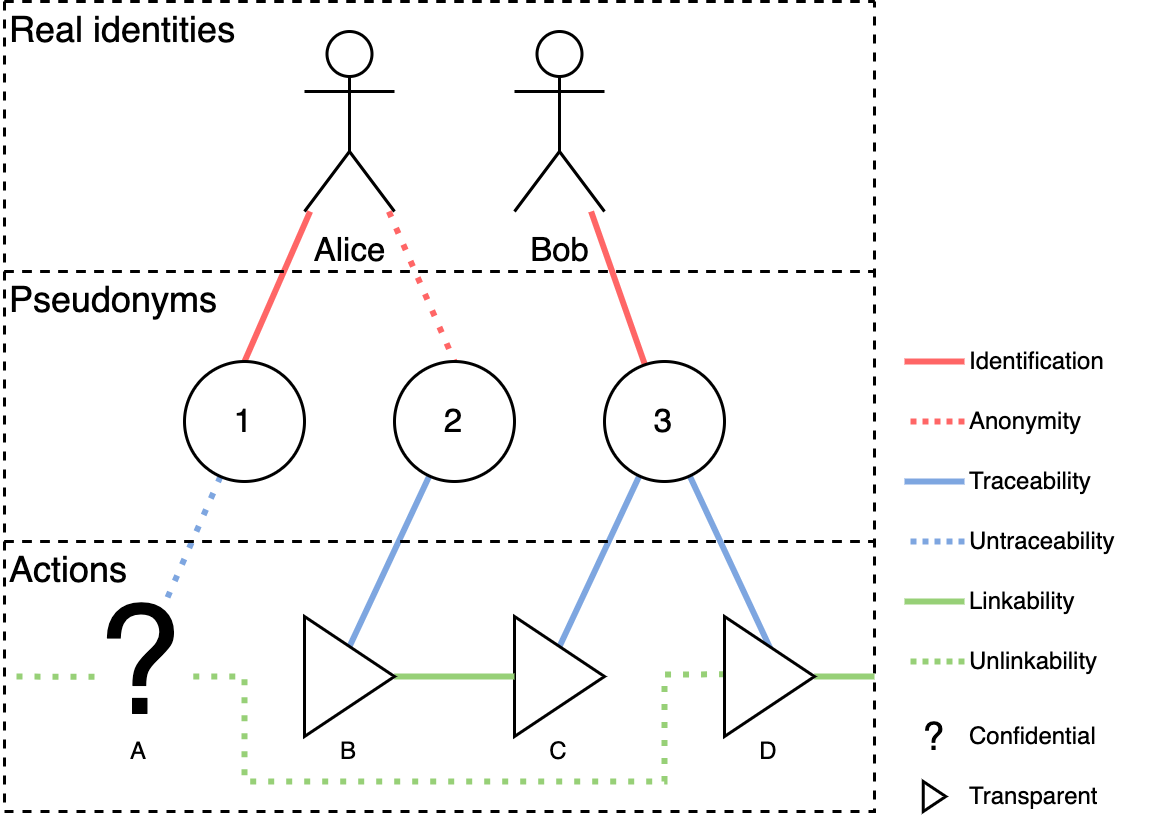
\includegraphics[width=\linewidth]{anonymity-diagram.png}
\centering
\caption{Suppose Alice is the client who wants to keep her identity anonymous and Bob is the public SP. Alice controls two addresses 1 and 2; the link between her real identity and the first address has been compromised and therefore identification is possible; the link to the second pseudonym is still unknown and therefore anonymous. Alice takes two actions, the first from the compromised address and the second from the anonymous address. The first action is confidential; therefore, even though the pseudonym has been compromised, the action cannot be associated with Alice. The second action is transparent, so Alice maintains her anonymity as long as the link to the second pseudonym is concealed.}

\label{fig:anonymity-diagram}
\end{figure}
The privacy-preserving blockchains are those that maintain anonymity through untraceability and (ideally) unlikability - not by assuming that the link between an address (pseudonym) and real identity is hidden.   

Examples of blockchains that natively support confidential transactions include Monero~\cite{vansaberhagenCryptoNote2013} (using Ring Signatures~\cite{noetherRingSignatureConfidential2015} or Bulletproofs~\cite{bunzBulletproofsShortProofs2018}), ZCash~\cite{ben-sassonZerocashDecentralizedAnonymous2014} (using zkSNARK~\cite{ben-sassonSNARKsVerifyingProgram2013}), Grin~\cite{fuchsbauerAggregateCashSystems2019} (using Mimblewimble~\cite{jedusorMIMBLEWIMBLE2016}), and IronFish~\cite{ironfishPrivateAnonymousEasy} (using Sapling protocol~\cite{hopwoodZcashSaplingProtocol2022}).

Overly techniques that achieve anonymity on top of non-privacy preserving blockchains are Ethereum's Tornado Cash~\cite{pertsevTornadoCashPrivacy2019} (via zkSNARK~\cite{grothSizePairingbasedNoninteractive2016} and MiMC~\cite{albrechtMiMCEfficientEncryption2016}), Bitcoin's Wasabi~\cite{wasabiwalletBitcoinPrivacyWallet} (via CoinJoin~\cite{maxwellCoinJoinBitcoinPrivacy2013}).

\subsection{Payment for services}\label{payment-for-services}
Transactions between customers and SPs need to be linked to prevent the reuse of a payment for multiple transactions. In other words, we need a mechanism that uniquely links the payment to the corresponding transaction.

Depending on the cryptocurrency, this link can be established in different ways:

\begin{itemize}
\item separate address: each transaction uses a unique address associated with the transaction. Such addresses can be derived using Hierarchical Deterministic Wallets~\cite{wuilleBIP32HierarchicalDeterministic2012} and published on the message board to achieve non-repudiation.
\item memo: payments are sent to a single SP account, but contain an extra field called ``memo'' filled with the unique identifier $\textrm{provisionID}$. 
\end{itemize}

Any payment that contains $\textrm{provisionID}$ in the memo or is sent to the designated address will be considered payment for the transaction. 

In the event of a dispute, there must be a way to prove to the courts that the customer has paid for the transaction. As proof of payment is trivial in transparent and traceable blockchains, it becomes more complicated when it comes to anonymous blockchains. Monero allows payments to be proven and verified via a dedicated API~\cite{moneroHowProvePayment}. ZCash provides a mechanism called Payment Disclosure~\cite{daviesIntroductionPaymentDisclosure2017}. We call the proof of payment a \textit{payment recepit}.

\subsection{Storage network}\label{storage-network}
Once the SP finishes its service, she has to provide the result to the customer. The most natural approach would be to send the result via e-mail or some dedicated platform. However, the customer wants to stay anonymous and so does not want to expose his e-mail address nor IP address. Moreover, the SP should prove that the result has been provided before the deadline, which brings us to the issue of proof of existence discussed in Section ~\ref{sec:message-board}.

One approach would be to post the result into a blockchain. However, storing data on a blockchain is very expensive. The most common workaround (\cite{shahidBlockchainBasedAgriFoodSupply2020, wangAuditableProtocolsFair2019, chenImprovedP2PFile2017}) is to publish the data on a content addressable peer-to-peer storage network like IPFS~\cite{benetIPFSContentAddressed2014}. Then, publish on the blockchain just the content identifier ($\mathrm{cid}$) that uniquely points to the content stored on IPFS.

We take the same approach. Once the SP creates the result, she encrypts it using the previously provided encryption key and uploads it to the IPFS network.
%TODO: write about DHKE encyption

To increase anonymity, the customer should use standard techniques to hide its IP address, such as VPN, or proxy.

\subsection{Separation of concerns}
We could use one blockchain to achieve all of these three roles: (i) anonymous payments, (ii) message board, (iii) storage network.

While most blockchains could provide message board functionality, anonymous payments are not as common. Especially a provable storage network is a functionality of a few specialized blockchains.

Instead of searching for one blockchain that provides all the functionalities, we allow the protocol to use separate blockchains for each role. If a suitable blockchain arises, it can play more than one role.

At the time of writing, we see the following technologies that fulfill the requirements of each role:

\begin{enumerate}
\def\labelenumi{\arabic{enumi}.}

\item Anonymous payments: Monero \cite{vansaberhagenCryptoNote2013}, ZCash
  \cite{ben-sassonZerocashDecentralizedAnonymous2014}, Grin \cite{fuchsbauerAggregateCashSystems2019},
  Tornado Cash \cite{pertsevTornadoCashPrivacy2019}.
\item Message board: Open timestamps~\cite{opentimestampsTimestampingProofStandard}, Stampery \cite{crespoStamperyBlockchainTimestamping2017}, Bitcoin blockchain (Proof of Existence~\cite{proofofexistenceWebApplicationProve}, Chainpoint~\cite{chainpointBlockchainProofAnchoring}), Ethereum blockchain, or any other public blockchain that supports attaching extra data along the transaction.
\item Storage network: IPFS~\cite{benetIPFSContentAddressed2014}, Filecoin~\cite{protocollabsFilecoinDecentralizedStorage2017}, or Ethereum's
  Swarm~\cite{teamSWARMStorageCommunication2021}.
\end{enumerate}

\section{The Protocol}\label{sec:protocol}
In this section, we propose an abstract protocol for anonymous service provisioning without any assumptions about the underlying technologies. We define the requirements for each role and leave the choice of the technology to the developer. Later in the paper (Section~\ref{sec:experiments}) we describe our implementation used to conduct an experiment.

\subsection{Assumptions}

\begin{itemize}
\item There exists PKI infrastructure:
    \begin{itemize}
        \item The customer and the SP have their key pairs consisting of secret key $\mathrm{sk}(\mathrm{party})$ and public key $\mathrm{pk}(\mathrm{party})$, where $\mathrm{party} \in \{\mathrm{C}, \mathrm{SP}\}$ for the customer and the SP accordingly.
        \item Both the customer and the SP can create and verify digital signatures created by the customer $\mathrm{sig}_{\mathrm{sk}(\mathrm{C})}$ and the SP $\mathrm{sig}_{\mathrm{sk}(\mathrm{SP})}$.
        \item The SP's public key $\mathrm{pk}(\mathrm{SP})$ is publicly known.
    \end{itemize}
    
\item Both the customer and the SP:
    \begin{itemize}
        \item use common symmetric encryption $\mathrm{E}_\mathrm{key}(\cdot)$ and decryption $\mathrm{D}_\mathrm{key}(\cdot)$ operations.
        \item have access to anonymous payments blockchain, message board, and storage network.
    \end{itemize}

\item The SP:
    \begin{itemize}
        \item accepts packages from unknown customers.
        \item accepts payments with cash and anonymous cryptocurrencies as described in Section~\ref{payment-for-services}.
    \end{itemize}
    
\item Justice:
    \begin{itemize}
        \item accepts as evidence in a dispute the $\mathrm{PoD}$, $\mathrm{PoP}$, and payment $\mathrm{receipt}$ as described in Section~\ref{fairness}.
    \end{itemize}

\item Anonymous payments blockchain:
    \begin{itemize}
        \item supports anonymous, i.e., untraceable and (ideally) unlinkable transactions as specified in Section~\ref{sec:pseudo-anon}.
        \item supports uniquely identifying transactions via a dedicated address, memo field, or other similar mechanisms as described in Section ~\ref{payment-for-services}. 
    \end{itemize}

\item Message Board:
    \begin{itemize}
        \item supports transactions of sizes up to $\mathrm{PoD}$ and $\mathrm{PoP}$.
    \end{itemize}

\item Storage network:
    \begin{itemize}
        \item allows for content retrieval via content identifier $\mathrm{cid}$ (usually a hash of the content).
        \item allows for anonymous content retrieval.
        \item guarantee that the content will be available for the duration of the agreement.
    \end{itemize}
\end{itemize}

\subsection{Messages}\label{messages}
In this section, we describe the messages exchanged between the parties of the protocol.

\vspace{5mm}

\noindent \textbf
{Package}\label{package} is a physical container prepared by the customer encompassing all $\mathrm{materials}$ required by the SP to provide the service.

$$\mathrm{pkg} \equiv (\mathrm{materials}, \mathrm{provisionID}, \mathrm{pk(C)})$$

where:

\begin{itemize}

\item $\mathrm{materials}$ - are the materials required to provide the service, for example, samples of urine, blood, stool, saliva; legal documents, CDs, emails, photos, bank statements; or any other kind of materials depending on the service.
\item $\mathrm{provisionID}$ - a randomly generated provision identifier, used to anonymously track the provision throughout the protocol's steps.
\item $\mathrm{pk(C)}$ - customer's public key used to encrypt the result published on the public storage network.
\end{itemize}

\noindent \textbf
{Proof of delivery ($\mathrm{PoD}$)}\label{proof-of-delivery} is an attestation to the fact that the customer has delivered a correct (according to the SP requirements) package to the SP, and the SP has accepted it.

It is also an agreement between the customer and the SP, as it includes agreed upfront deadlines of actions and a payment method.

$\mathrm{PoD}$ is published on the message board by the SP.

\begin{eqnarray}
\mathrm{PoD} & \equiv & (\begin{array}[t]{l}\mathrm{T}_\mathrm{issue}, \mathrm{T}_\mathrm{pay}, \mathrm{T}_\mathrm{provide}, \\\\ \mathrm{address}, \mathrm{provisionID}, \mathrm{pk(C)}, \mathrm{sig}_\mathrm{SP} \; )\end{array}
\end{eqnarray}

where:

\begin{itemize}

\item $\mathrm{T}_\mathrm{issue}$ - time at which the $\mathrm{PoD}$ is issued by the SP.
\item
  $\mathrm{T}_\mathrm{pay}$ - deadline to pay for the transaction.
\item
  $\mathrm{T}_\mathrm{provide}$ - deadline to provide the result of the service, i.e. publish $\mathrm{PoP}$.
\item $\mathrm{address}$ - payment address of the SP's anonymous blockchain account.
\item $\mathrm{provisionID}$ - the number uniquely identifying the transaction previously generated by the customer.
\item $\mathrm{pk(C)}$ - customer's public key used to encrypt the result published on the public storage network.
\item $\mathrm{sig}_\mathrm{SP}$ - the SP's signature guaranteeing non-repudiation.
\end{itemize}

also:
\(\mathrm{T}_\mathrm{issue} \leq \mathrm{T}_\mathrm{pay} \leq \mathrm{T}_\mathrm{provide}\)

\noindent \textbf
{Proof of provision ($\mathrm{PoP}$)}\label{proof-of-provision} is proof that the SP published the result at a certain time. It protects the SP in case the customer unjustly starts a dispute after the result has been published. The connection between $\mathrm{PoP}$ and the result is made by the content identifier ($\mathrm{cid}$) uniquely identifying the result such that the result can not be forged after the $\mathrm{PoP}$ has been published.

$\mathrm{PoP}$ is published on the message board by the SP.


\begin{eqnarray}
\mathrm{PoP} & \equiv & (\mathrm{cid}, \mathrm{provisionID}, \mathrm{sig}_\mathrm{SP})
\end{eqnarray}

where:

\begin{itemize}

\item $\mathrm{cid}$ - content identifier as specified in Section~\ref{storage-network}.
\item $\mathrm{provisionID}$ - the number uniquely identifying the transaction previously generated by the customer.
\item $\mathrm{sig}_\mathrm{SP}$ - the SP's signature guaranteeing non-repudiation.
\end{itemize}

\noindent \textbf
{Payment receipt}\label{payment-receipt} proves that the customer did the payment. Since the evidence depends on a particular blockchain (see Section~\ref{payment-for-services}), we refer to it symbolically as
$\mathrm{receipt}$.

\noindent \textbf
{Result}\label{results} is assumed to be a document in PDF format, but any other format is allowed as long as it can be binary encoded and uploaded to the storage network. We refer to it symbolically as $\mathrm{result}$.

\noindent \textbf
{Content Identifier (cid)}\label{content-identifier-cid} is a term coined by IPFS~\cite{ipfsContentIdentifiersCIDs}. However, since our protocol does not depend on this particular implementation of the storage network, we let the $\mathrm{cid}$ be any other identifier that securely and uniquely points to the content.

\subsection{Protocol description}\label{protocol-description}

In this section, we describe each step of the protocol, also shown in the Figure~\ref{fig:protocol-diagram}.

\begin{figure}[ht!]
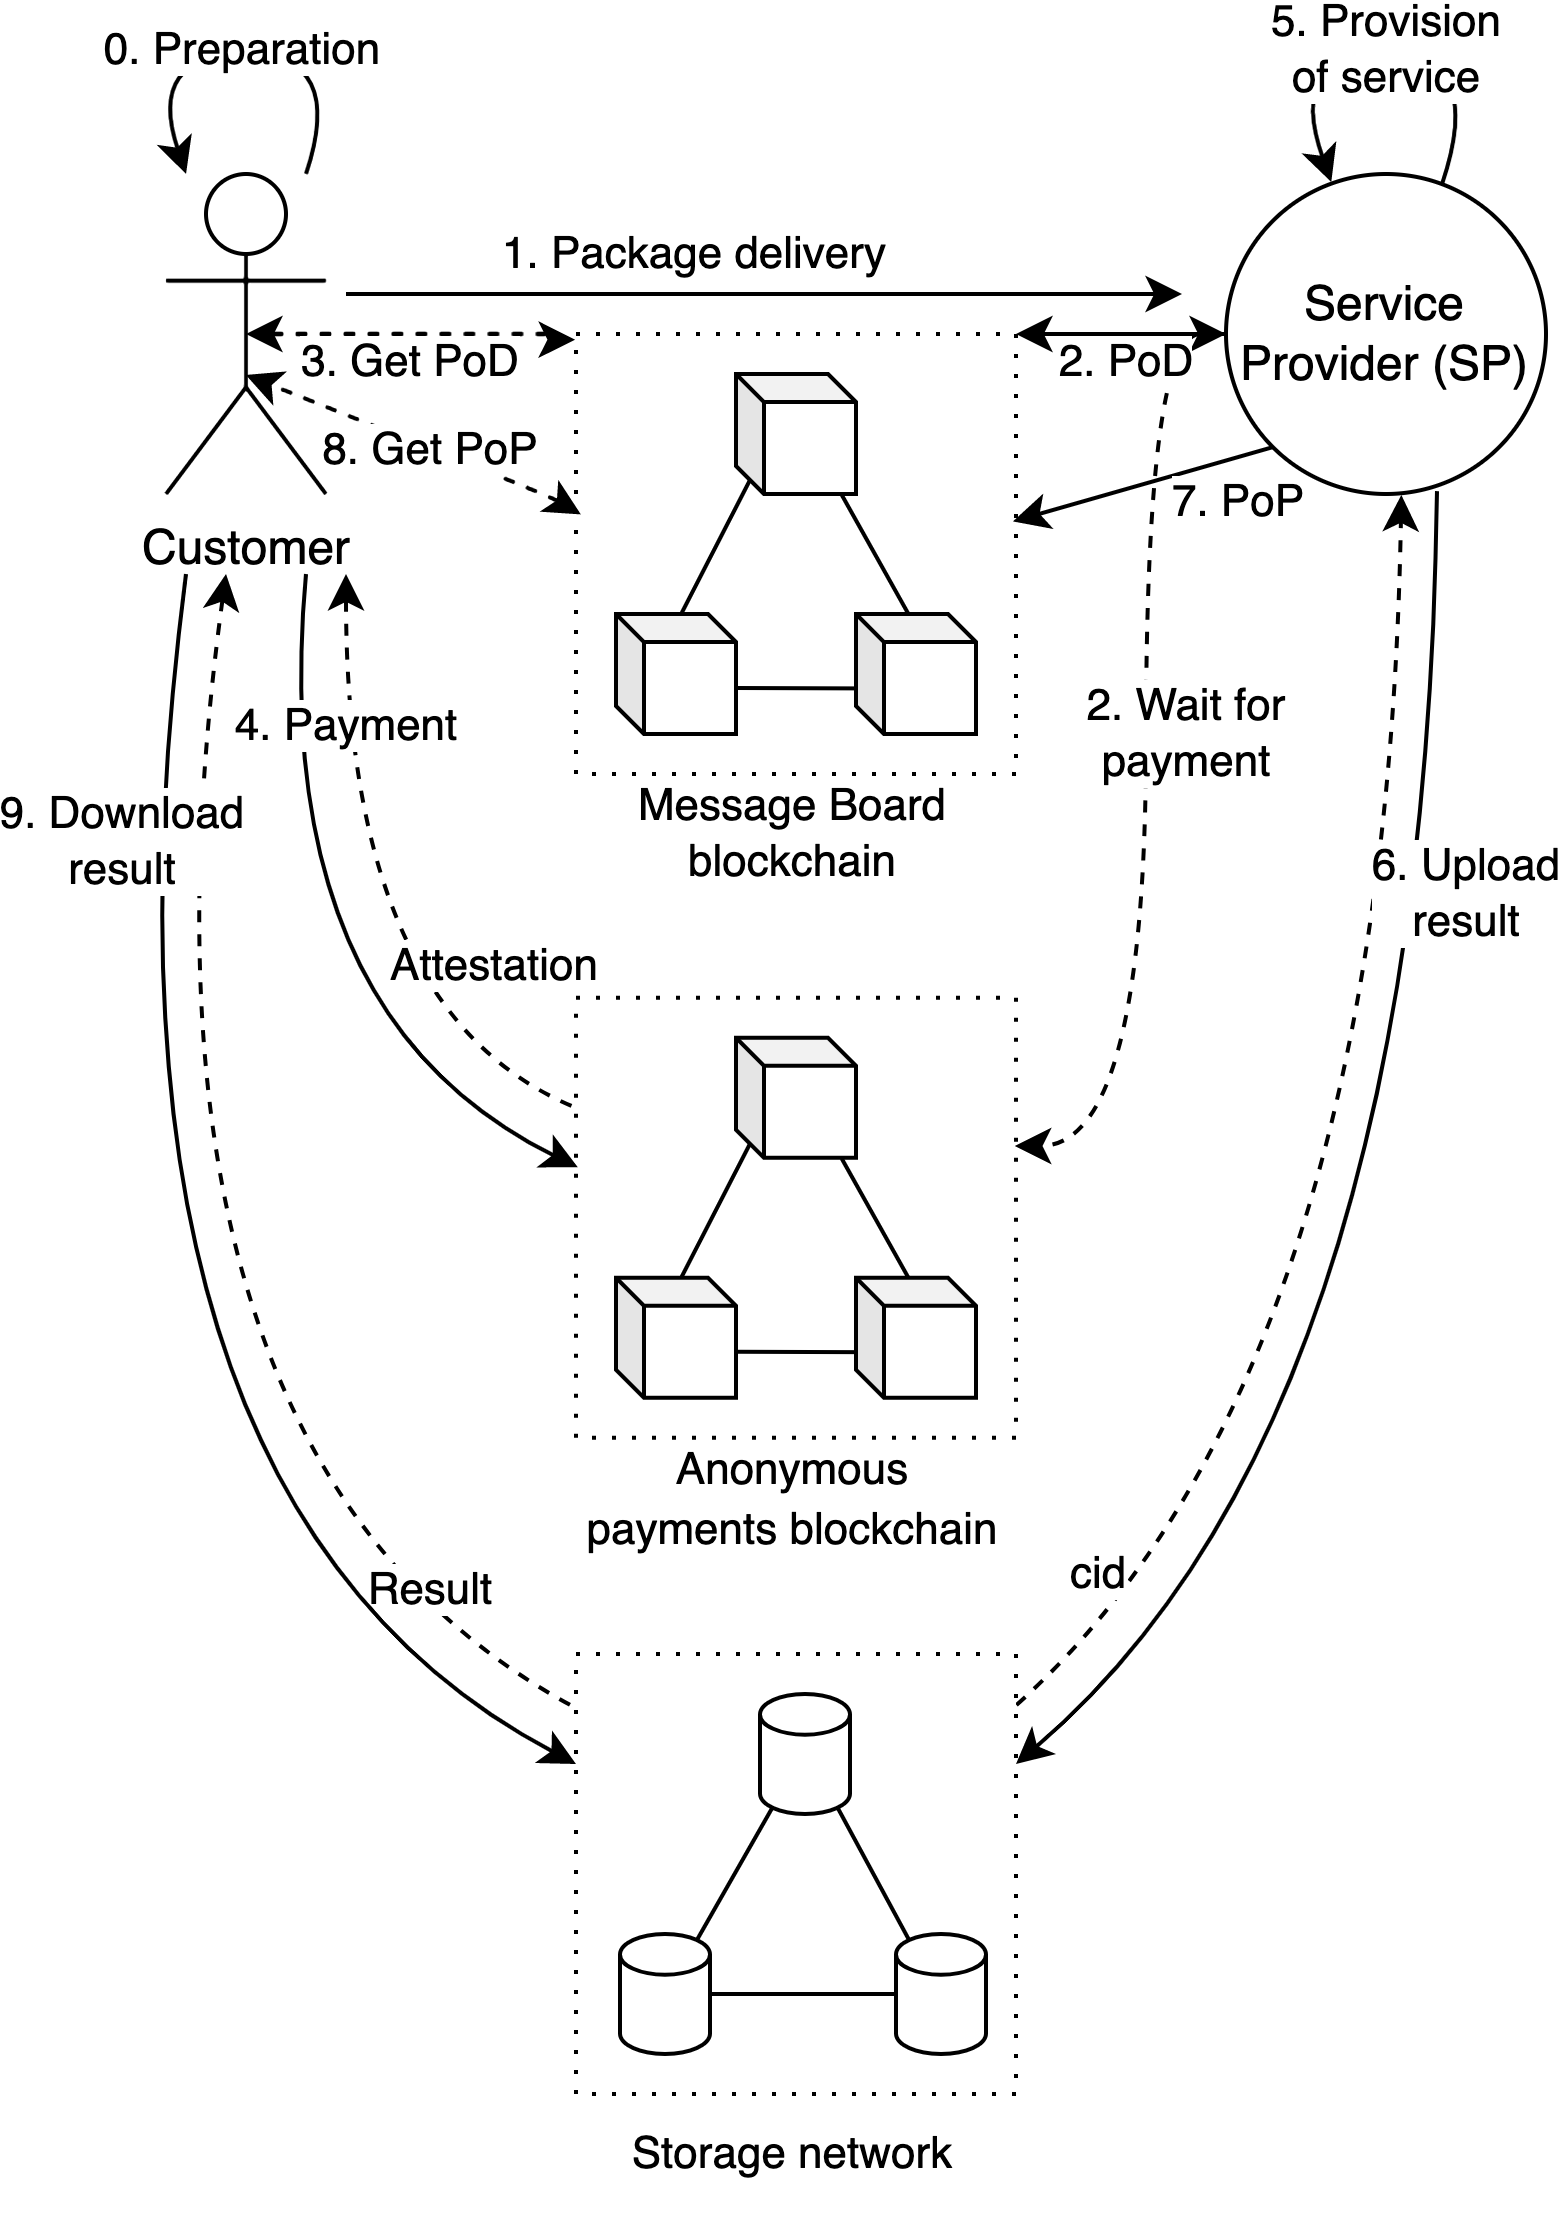
\includegraphics[width=\linewidth]{anonser-protocol.png}
\centering
\caption{Messages exchanged in the protocol. Solid arrows indicate requests and dashed arrows indicate responses.}
\label{fig:protocol-diagram}
\end{figure}

\noindent \textbf
{Step 0.  Preparation}\label{step-0-preparation}

The customer collects all the $\mathrm{materials}$ required by the SP, generates a random $\mathrm{provisionID}$ and a random keypair $(\mathrm{sk(C)},\mathrm{pk(C)})$. The $\mathrm{provisionID}$ will be used to associate all actions related to the transaction throughout the protocol. The $\mathrm{provisionID}$ and $\mathrm{pk(C)}$ are encoded as a QR code, printed, and stuck to the package $\mathrm{pkg}$. The $\mathrm{sk(C)}$ is kept secret and used to decrypt the $\mathrm{result}$ at the end of the protocol.

\noindent \textbf
{Step 1. Package delivery}\label{step-1-package-delivery}

The protocol starts once the customer delivers package $\mathrm{pkg}$ to the SP and its content gets accepted. As a result, $\mathrm{PoD}$ is created with predefined payment deadline $\mathrm{T}_\mathrm{pay}$, service provision deadline $\mathrm{T}_\mathrm{provide}$, and current time $\mathrm{T}_\mathrm{issue}$. Also, $\mathrm{PoD}$ embodies the information whether the service has been paid in cash or should be paid by the customer using the anonymous blockchain account. In the latter case, the SP's payment $\mathrm{address}$ is included in the $\mathrm{PoD}$.

The digital signature $\mathrm{sig}_{\mathrm{sk}(\mathrm{SP})}$ on the $\mathrm{PoD}$ created with the SP's secret key $\mathrm{sk}(\mathrm{SP})$ guarantee non-repudiation.

Symbolically: 
\[
\mathrm{PoD \gets delivery(pkg)}
\]

\noindent \textbf
{Step 2. Proof of Delivery}\label{step-2-pod}

Then, the $\mathrm{PoD}$ is published on the message board by the SP, committing to the fact that the package $\mathrm{pkg}$ has been delivered, and the SP can not reject receiving it. If the provision has not been paid in cash, the SP waits for the customer to pay for the service on the specified in the $\mathrm{PoD}$ payment $\mathrm{address}$.

Symbolically: 
\[
\mathrm{publish(PoD)}
\]

\noindent \textbf
{Step 3. Get Proof of Delivery}\label{step-3-get-pod}

Once the package is delivered and the $\mathrm{PoD}$ is published, the customer can get the $\mathrm{PoD}$ from the message board and (if everything is correct) proceed with the protocol.

Symbolically: 
\[
\mathrm{PoD \gets get(provisionID)}
\]

\noindent \textbf
{Step 4. Payment}\label{step-4-payment}

If the provision has not been paid in cash, the customer should pay for the transaction with the predefined anonymous payment blockchain (see Section~\ref{payment-for-services}).
In return, the customer receives the $\mathrm{receipt}$ that should be disclosed in case of a dispute.

Symbolically: 
\[
\mathrm{receipt \gets payment(address)}
\]

\noindent \textbf
{Step 5. Provision of service}\label{step-5-provision-of-service} 

Once the customer has paid for the transaction either in cash or using the anonymous blockchain, the SP can start providing the service.

Symbolically: 
\[
\mathrm{result \gets provision(materials)}
\]

\noindent \textbf
{Step 6. Upload result}\label{step-6-upload-result}

After the service is finished, a result should be created. 
Next, the result is encrypted using a shared key derived from the customer's public key $\mathrm{pk(C)}$ and the SP's secret key $\mathrm{sk(S)}$ using Diffie-Hellman key exchange (DHKE) method~\cite{diffieNewDirectionsCryptography1976}.
The encrypted result is then uploaded on the content addressable network (such as IPFS). In return, the content identifier ($\mathrm{cid}$) is created.

Symbolically: 
\[
\mathrm{cid \gets upload(E_{DHKE(sk(SP), pk(C))}(result))}
\]

\noindent \textbf
{Step 7. Proof of provision}\label{step-7-proof-of-provision}

When the $\mathrm{result}$ is uploaded, the SP creates and publishes on a message board a proof of provision consisting of $\mathrm{cid}$ along with $\mathrm{provisionID}$ and signature $\mathrm{sig}_\mathrm{SP}$.

Symbolically: 
\[
\mathrm{publish(PoP)}
\]

\noindent \textbf
{Step 8. Get Proof of Provision}\label{step-8-get-proof-of-provision}

After delivering the package and paying for the transaction, the customer starts listening to the message board and waits until the SP publishes the $\mathrm{PoP}$ for the $\mathrm{provisionID}$.

Symbolically: 
\[
\mathrm{cid \gets get(provisionID)}
\]

\noindent \textbf
{Step 9. Download result}\label{step-9-download-result}

Having the $\mathrm{cid}$, the customer downloads and decrypts the $\mathrm{result}$ using a shared key derived from the customer's secret key $\mathrm{sk(C)}$ and the SP's public key $\mathrm{pk(S)}$ using DHKE method. The protocol ends.

Symbolically: 
\[
\mathrm{result \gets D_{DHKE(sk(C), pk(SP))}(download(cid))}
\]

\section{Fairness analysis}\label{sec:fairness-analysis}
We analyze the fairness of the protocol by representing it as an interactive non-cooperative game.

\subsection{Model}\label{sec:fairness-model}
We consider three positions:

\begin{itemize}
\item Neutral position (•): when a party has not spent nor gained anything of significant value (money, time, effort). For example, at the beginning of the protocol.
\item Disadvantaged position (-): when a party has put a significant value without receiving an equivalent. For example, the customer has paid for a service in advance.
\item Advantaged position (+): when a party would benefit if the transaction would halt at that step. For example, the SP has received payment before service provision.
\end{itemize}

There are many actions that each party can take, but we group them into two categories:

\begin{enumerate}
\def\labelenumi{\arabic{enumi}.}

\item Normal: taking actions prescribed by the protocol.
\item Abnormal: everything that deviates from the designed steps of the protocol. For example, sending an arbitrary message, skipping or repeating steps, and timing out.
\end{enumerate}

Moreover, at any step of the protocol, the customer can start a dispute; therefore, another dimension with two positions has to be considered:

\begin{enumerate}
\def\labelenumi{\arabic{enumi}.}

\item Agree: the customer agrees with the action and therefore does not start a dispute.
\item Start a dispute: the customer disagrees with the action and therefore starts a dispute.
\end{enumerate}

As a result, in our analysis, we have to consider four different outcomes for each party of the protocol ($\mathrm{party \in \{c, s}\}$), for each step of the protocol ($\mathrm{step \in 1..9}$):

\begin{itemize}

\item
  $\mathrm{\sigma_{step,party,n}}$: after following the protocol when the other party acted normally.
\item
  $\mathrm{\sigma_{step,party,d}}$: after a settled dispute when the other party acted normally.
\item
  $\mathrm{\sigma_{step,party,\overline{n}}}$: after not starting a dispute despite the other party has acted abnormally.
\item
  $\mathrm{\sigma_{step,party,\overline{d}}}$: after a settled dispute when the other party has acted abnormally.
\end{itemize}



The protocol terminates after the last step, after starting a dispute, or after a party has not completed its designated action in time. Therefore, all positions but $\mathrm{\sigma_n}$ are termination positions.

Because the customer is anonymous, the SP can not start a dispute—there is no means to identify the customer. To mitigate the issue, we designed the protocol so that the SP who follows the protocol is always in an advantaged position, and therefore has no reason to start a dispute. On the other hand, the customer can start a dispute at any time of the protocol, but only the actual misbehavior of the SP makes him win the conflict.

\begin{definition}[Fairness] \label{def:fairness}
A protocol achieve fairness iff 
\begin{equation*}
\begin{split}
\forall_{party \in parties}\forall_{\mathrm{step} \in \mathrm{steps}} &\operatorname{can\ move}\\
&\operatorname{to\ the\ non-disadvantaged\ position} 
\end{split}
\end{equation*}

\end{definition}


\subsection{Assumptions}\label{sec:assumptions}

Below we list the assumptions we take for the analysis purpose.  

\begin{enumerate}
\item Both parties start from a neutral position $\neutral$.
\item After completing a transaction, both parties end up in advantaged positions (\plus{}). In other words, they have an intrinsic motivation to initialize and complete the transaction.
\item The protocol steps are atomic—there are no intermediate steps.
\item The protocol can go only forward—there is no way of reverting any action.
\item Repeating the first step starts a new transaction. Repeating any other step is considered abnormal and gets ignored. For example, paying for the invoice twice does not cause any effect on the curse of the protocol.
\item Once published, the result is available to the customer on the storage network. The idea of guaranteeing it cryptographically is discussed in Section~\ref{sec:discussion}.
\item Winning the dispute leads to a neutral position ($\neutral$).
\item Losing the dispute leads to a punishment greater than any reward, leading to a disadvantaged position (\minus{}). Hence, the rational customer will not start a dispute that he is unsure of winning.
\item Both the customer and the SP are rational (selfish). They always prefer to go from the worst position (\minus{} or $\neutral${}) to a better position ($\neutral$ or \plus), but also risk a temporary worst position in favor of a later better position if and only if at any time they can get out of the worst position; in particular, at any time the customer can start a dispute and, if the SP has misbehaved, get out of disadvantaged position (\minus) to the neutral position ($\neutral$).
\item We assume that the Customer's materials without personal information are useless, and the effort to deliver the package is negligible, so that the Customer's first step does not lead to disadvantaged position.
\item We assume the processing cost of publishing $\mathrm{PoD}$ is negligible and balance out the effort of delivering the package by the Customer.
\end{enumerate}

\subsection{Steps}\label{sec:steps}

Figure~\ref{fig:positions} shows the positions of each party after each possible action taken.

\begin{figure}[h!]
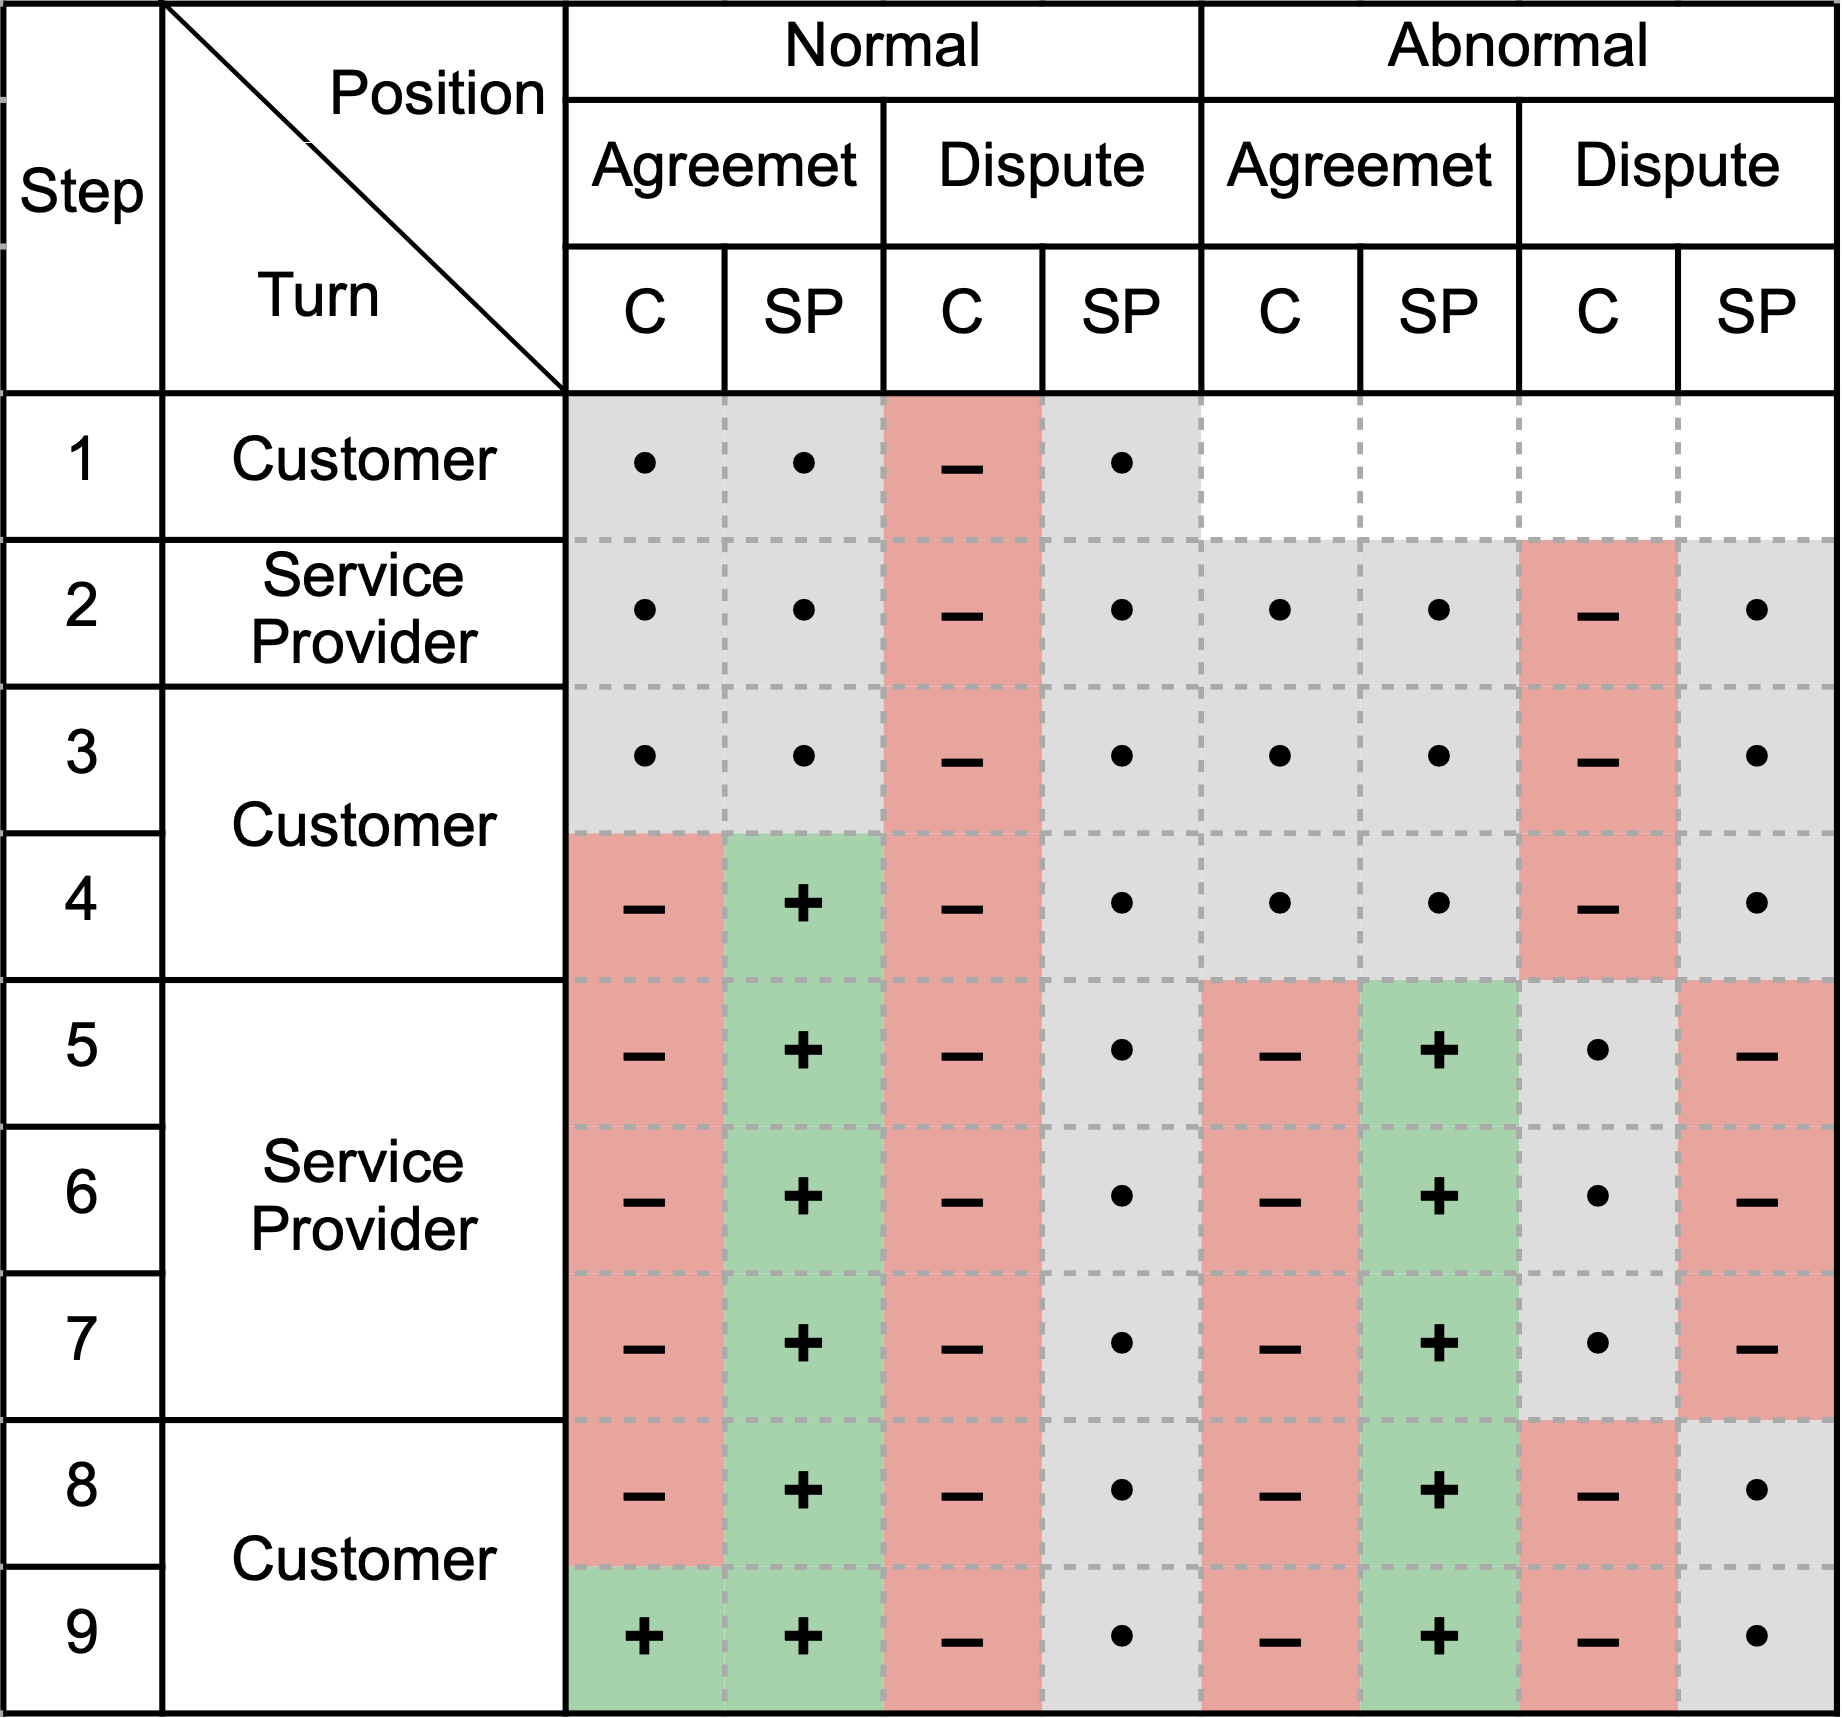
\includegraphics[width=\linewidth]{model.png}
\centering
\caption{Positions after each step of protocol}
\label{fig:positions}
\end{figure}

The detailed description of each step and the justification
of the outcome positions is given in Appendix~\ref{app:proof-of-fairness}.

\subsection{Example scenarios}\label{example-scenarios}

The Figure~\ref{fig:misbehaviour} shows the transitions of positions when the SP tries to misbehave and does not execute service, and so does not publish $\mathrm{PoP}$ after receiving the payment. After the deadline $\mathrm{T}_\mathrm{provide}$ the SP can not publish valid $\mathrm{PoP}$ and so the Customer starts a dispute. The Customer wins the dispute as the SP is unable to proof the $\mathrm{PoP}$ was published before $\mathrm{T}_\mathrm{provide}$. The protocol ends up neutral to the customer and disadvantaged to the SP positions.

\begin{figure}[h!]
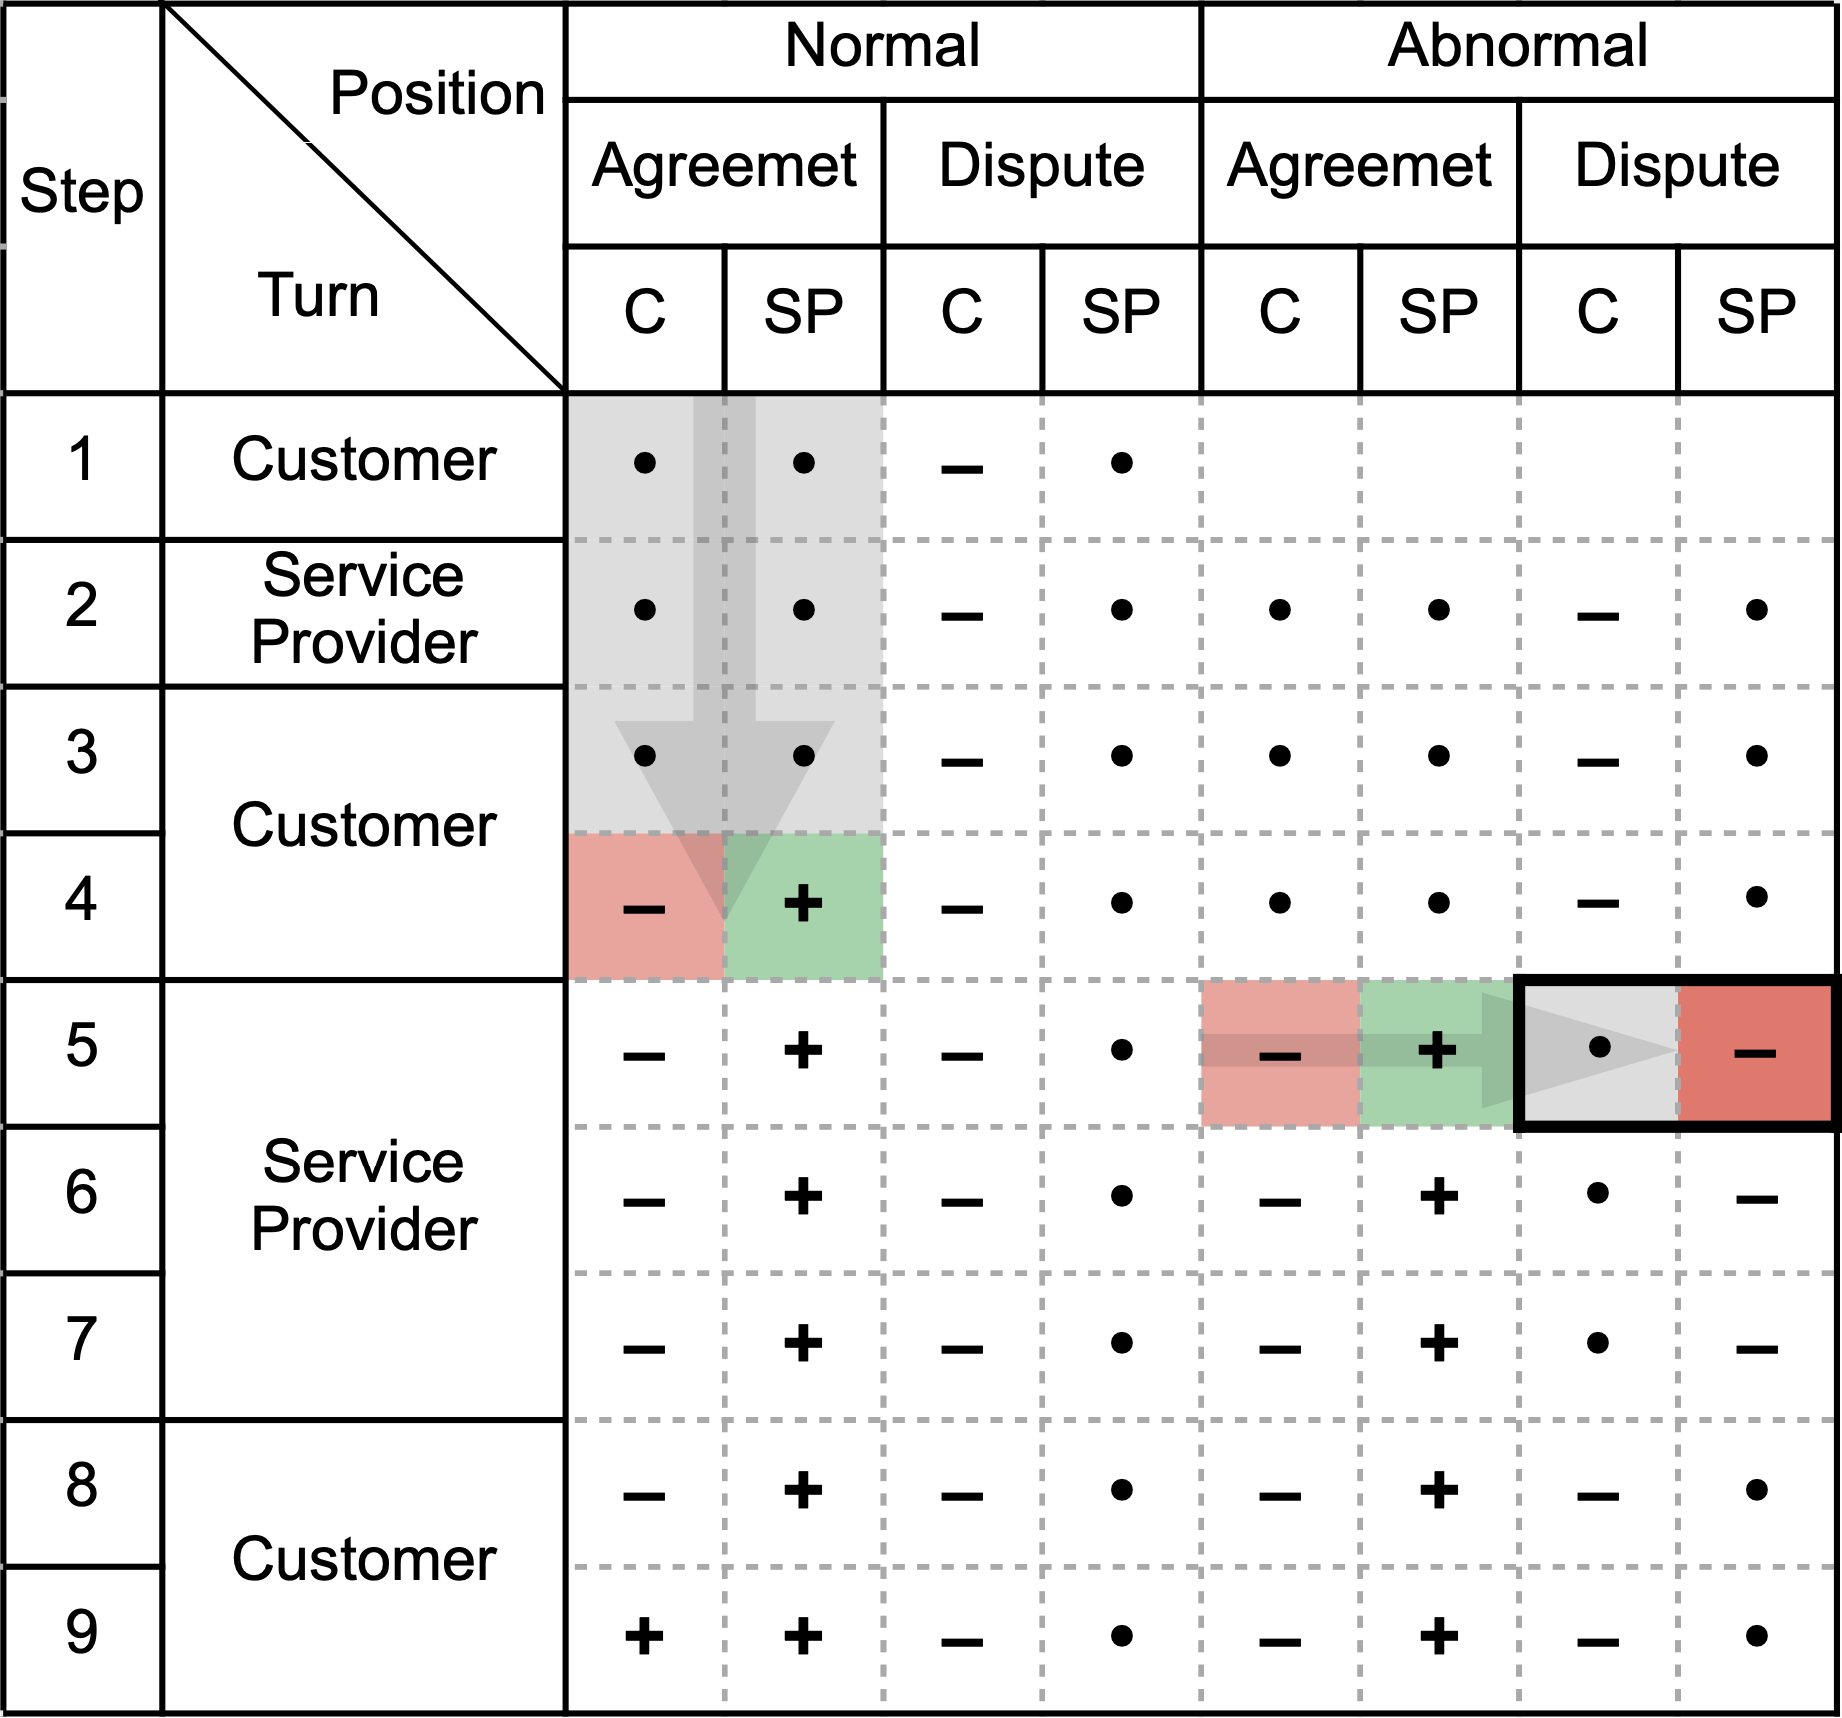
\includegraphics[width=\linewidth]{misbehaviour.png}
\centering
\caption{Transitions of positions where the SP is misbehaving and the customer starts a dispute}
\label{fig:misbehaviour}
\end{figure}
the rational path for both parties is to follow the protocol as shown in the Figure~\ref{fig:rational}.

\begin{figure}[h!]
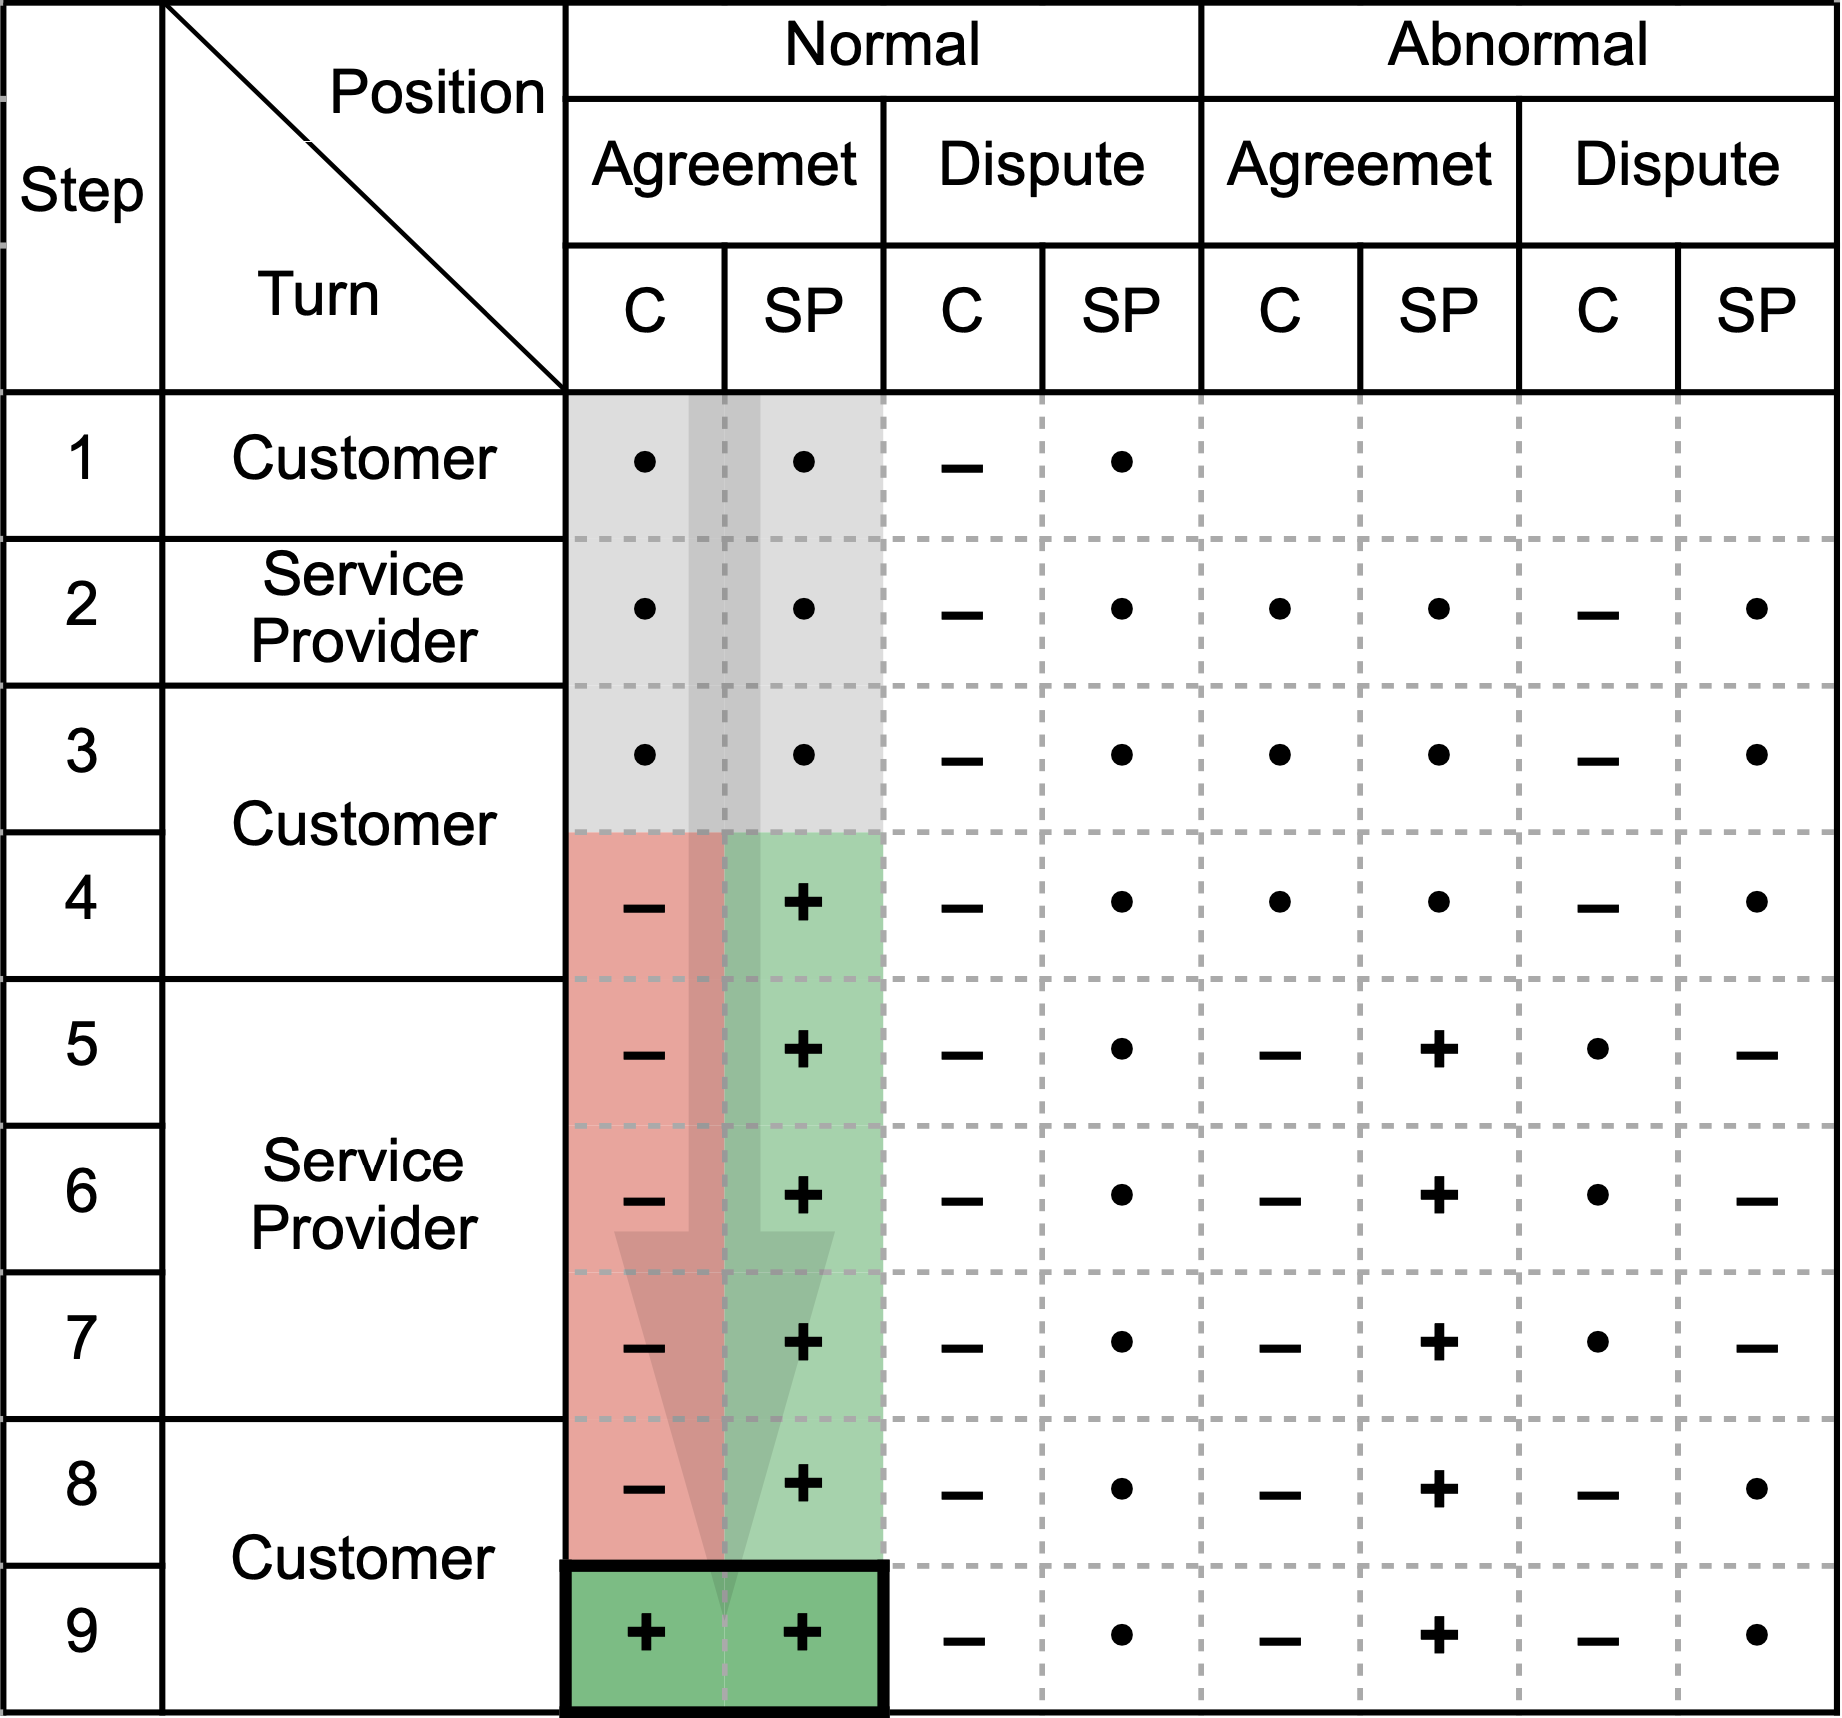
\includegraphics[width=\linewidth]{rational.png}
\centering
\caption{Transitions of positions where both the customer and the SP are following the protocol}
\label{fig:rational}
\end{figure}

Using the fairness definition~\ref{def:fairness} and the assumptions stated in Section~\ref{sec:assumptions}, our analysis indicates that the protocol achieves fairness.

\section{Experiments}\label{sec:experiments}

\subsection*{Setup}

We have developed a prototype of our protocol using the following technologies:

\begin{itemize}
  \item{Anonymous payments} — we use the Monero blockchain \cite{noetherRingSignatureConfidential2015}.
  \item{Storage netowork} — we use the Powergate~\cite{textilePowergate2023}, which is a wrapper around Filecoin and IPFS.
  \item{Message board} — we use the Ethereum blockchain \cite{woodEthereumSecureDecentralised2014}; concretely, its local development version Truffle Ganache and Solidity language.
  \item{Customer and SP} — we create client side web application (webapp) using \texttt{React.js} for creating UI, and \texttt{web3.js} library for interaction with Ethereum. We use \texttt{MetaMask} browser extension for signing and submitting transactions to Ethereum's node. We use \texttt{monerod} network client and \texttt{monero-wallet-cli} command-line interface for interacting with Monero blockchain.
\end{itemize}

The prototype is available at [blinded for review process]. The source code is available at [blinded for review process].

% The prototype is available at \url{https://anonser.stan.bar}. The source code is available at \url{https://github.com/stanbar/anonymous-provision-of-services-via-blockchain}.

We developed and tested our prototype in the following environment: OS — Arch Linux 5.11.8; Docker — 20.10.5; CPU — Intel(R) Core(TM) i7-4790 (8) 4.00~GHz; RAM — 16 GB DDR3; Storage — Samsung PM85 256~GB SSD; monerod and monero-wallet-cli — v0.18.1.2; Powergate — v2.6.2; Ganache — v7.5.0; Solidity — v0.8.17; ReactJS — v18.0.25; web3.js — v1.8.1; crypto-js — v4.1.1.

For simplicity, all components run on one, mentioned above, physical machine; and all processes are managed by Docker. 

Moreover, Powergate is configured to use local Filecoin and IPFS networks.
For Ethereum blockchain, we use Truffle Ganache, which is a local Ethereum blockchain for development and testing purposes. 
Monero is configured to use the public stage network.
We assume the service provider offers only one type of service, which is offered for a fixed public price, hence we omit the type of service and price from the protocol.

\subsection*{Preparation}

Both the customer and the SP create Monero wallets using \texttt{monero-wallet-cli} command-line tool.

The service provider deploys the smart contract using the \texttt{truffle migrate --network development} command, which deploys the smart contract to the Ethereum blockchain. The webapp is configured to use the latest deployed smart contract address.

The customer gets some testing Monero funds using faucet service available at \url{https://community.rino.io/faucet/stagenet/}.

Next, the customer enables per-transaction proof generation (payment \texttt{receipt}) by setting \texttt{set store-tx-info 1} for his wallet. Proof generation is required to verify the payment in case of a dispute.

At this point, both the customer and the SP are ready to start the protocol.

\subsection*{Experiment}

The customer and the SP are two different users of our prototype, but for simplicity, they use the same machine and the same web application.

Figures \ref{fig:anonser-experiment1} and \ref{fig:anonser-experiment2} show the steps of the experiment. Their description is as follows:

\begin{enumerate}
  \setcounter{enumi}{0}
  \item[0.] The protocol starts with the customer opening the webapp and creating a new provision. 
The app generates a random ECDSA (secp256k1) customer's keypair and random 32 bytes provisionID, then display QR code that encodes both the provisionID and the customer's public key. 
The customer's private key must be downloaded and provided later for the decryption of the results.

  \item[1.] The customer prints the QR code, sticks it on a package and delivers the package to the SP either: in person, via a trusted party, or a delivery agency.

  \item[2.1.] The SP opens the app, and scans the QR code decoding the provisionID and the client's public key.

  \item[2.2.] Since (in this experiment) the provision has not been paid in cash, the SP generates a unique Monero payment address using \texttt{monero-wallet-cli integrated\_address} 
  \item[2.3.] The SP submits the proof of delivery to the Ethereum blockchain using MetaMask interface. 

  % monero-wallet-cli --stagenet --wallet-file sp --password "" integrated_address
  % Random payment ID: <2b6d65d7d48b7896>
  % Matching integrated address: 5LHmrsVsQM2Q2TgqufX4A5gKPpxy1czHULDyVc84omvnh1nQLVmqXk4VBuy8WnX1AXfKxDx7xuASAc6svkZqGVkL1XkUBWT7QejHymEaYM
  \item[3.] The customer (using the webapp) checks the transaction status on the Ethereum blockchain invoking \texttt{getProvision} with arguments \texttt{customerPubKey} and \texttt{provisionID}.
  % monero-wallet-cli --stagenet --wallet-file customer --password "" transfer 5LHmrsVsQM2Q2TgqufX4A5gKPpxy1czHULDyVc84omvnh1nQLVmqXk4VBuy8WnX1AXfKxDx7xuASAc6svkZqGVkL1XkUBWT7QejHymEaYM 1
  % Transaction successfully submitted, transaction <7d89c04de458cfb76a811d5eb325075dec59f7a993c3bf7ce37f9e3a1630af65>
  % monero-wallet-cli --stagenet --wallet-file customer --password "" get_tx_key 7d89c04de458cfb76a811d5eb325075dec59f7a993c3bf7ce37f9e3a1630af65
  % Tx key: 1364dc848a752bf52011f4a63d98bcb16091cacd985713b6b5264b3ede6de40f

  \item[4.] The customer (using the \texttt{monero-wallet-cli transfer}) sends the payment to the designated in the smart contract \texttt{paymentAddress} and stores the payment receipt (using \texttt{monero-wallet-cli get\_tex\_key <tx-id>}) in case of a dispute.

  \item[5.] Once SP notices the payment on Monero blockchain it starts providing the service and outputs the file \texttt{result.pdf}.

  \item[6.] The SP uploads the file \texttt{result.pdf} on the Filecoin and IPFS networks using Powergate. As a result, the SP gets the content identifier \texttt{cid}, and \texttt{dealID} and \texttt{minerID}.

  \item[7.] The SP submits a Proof of Provision transaction to the Ethereum blockchain by invoking \texttt{proofOfProvision} with arguments \texttt{customer\-PubKey}, \texttt{provisionID}, \texttt{cid}, and \texttt{dealID}.

  \item[8.] Meantime, the Customer subscribes to Ethereum and waits until the SP publishes the Proof Of Provision.
 Once the Proof Of Provision is published the Customer downloads the result using either: IPFS network via \url{https://dweb.link/<cid>} or Lotus network using \texttt{lotus retrieve <cid> <minerID>}. 
 
  \item[9.] Results are then decrypted using the previously stored customer's private key. If everything is correct, the Customer is satisfied with the service and the protocol ends, otherwise, the Customer can initiate a dispute.

\end{enumerate}



\ifx\FORMAT\SINGLECOLUMN
\noindent%
\begin{minipage}{\linewidth}
\makebox[\linewidth]{
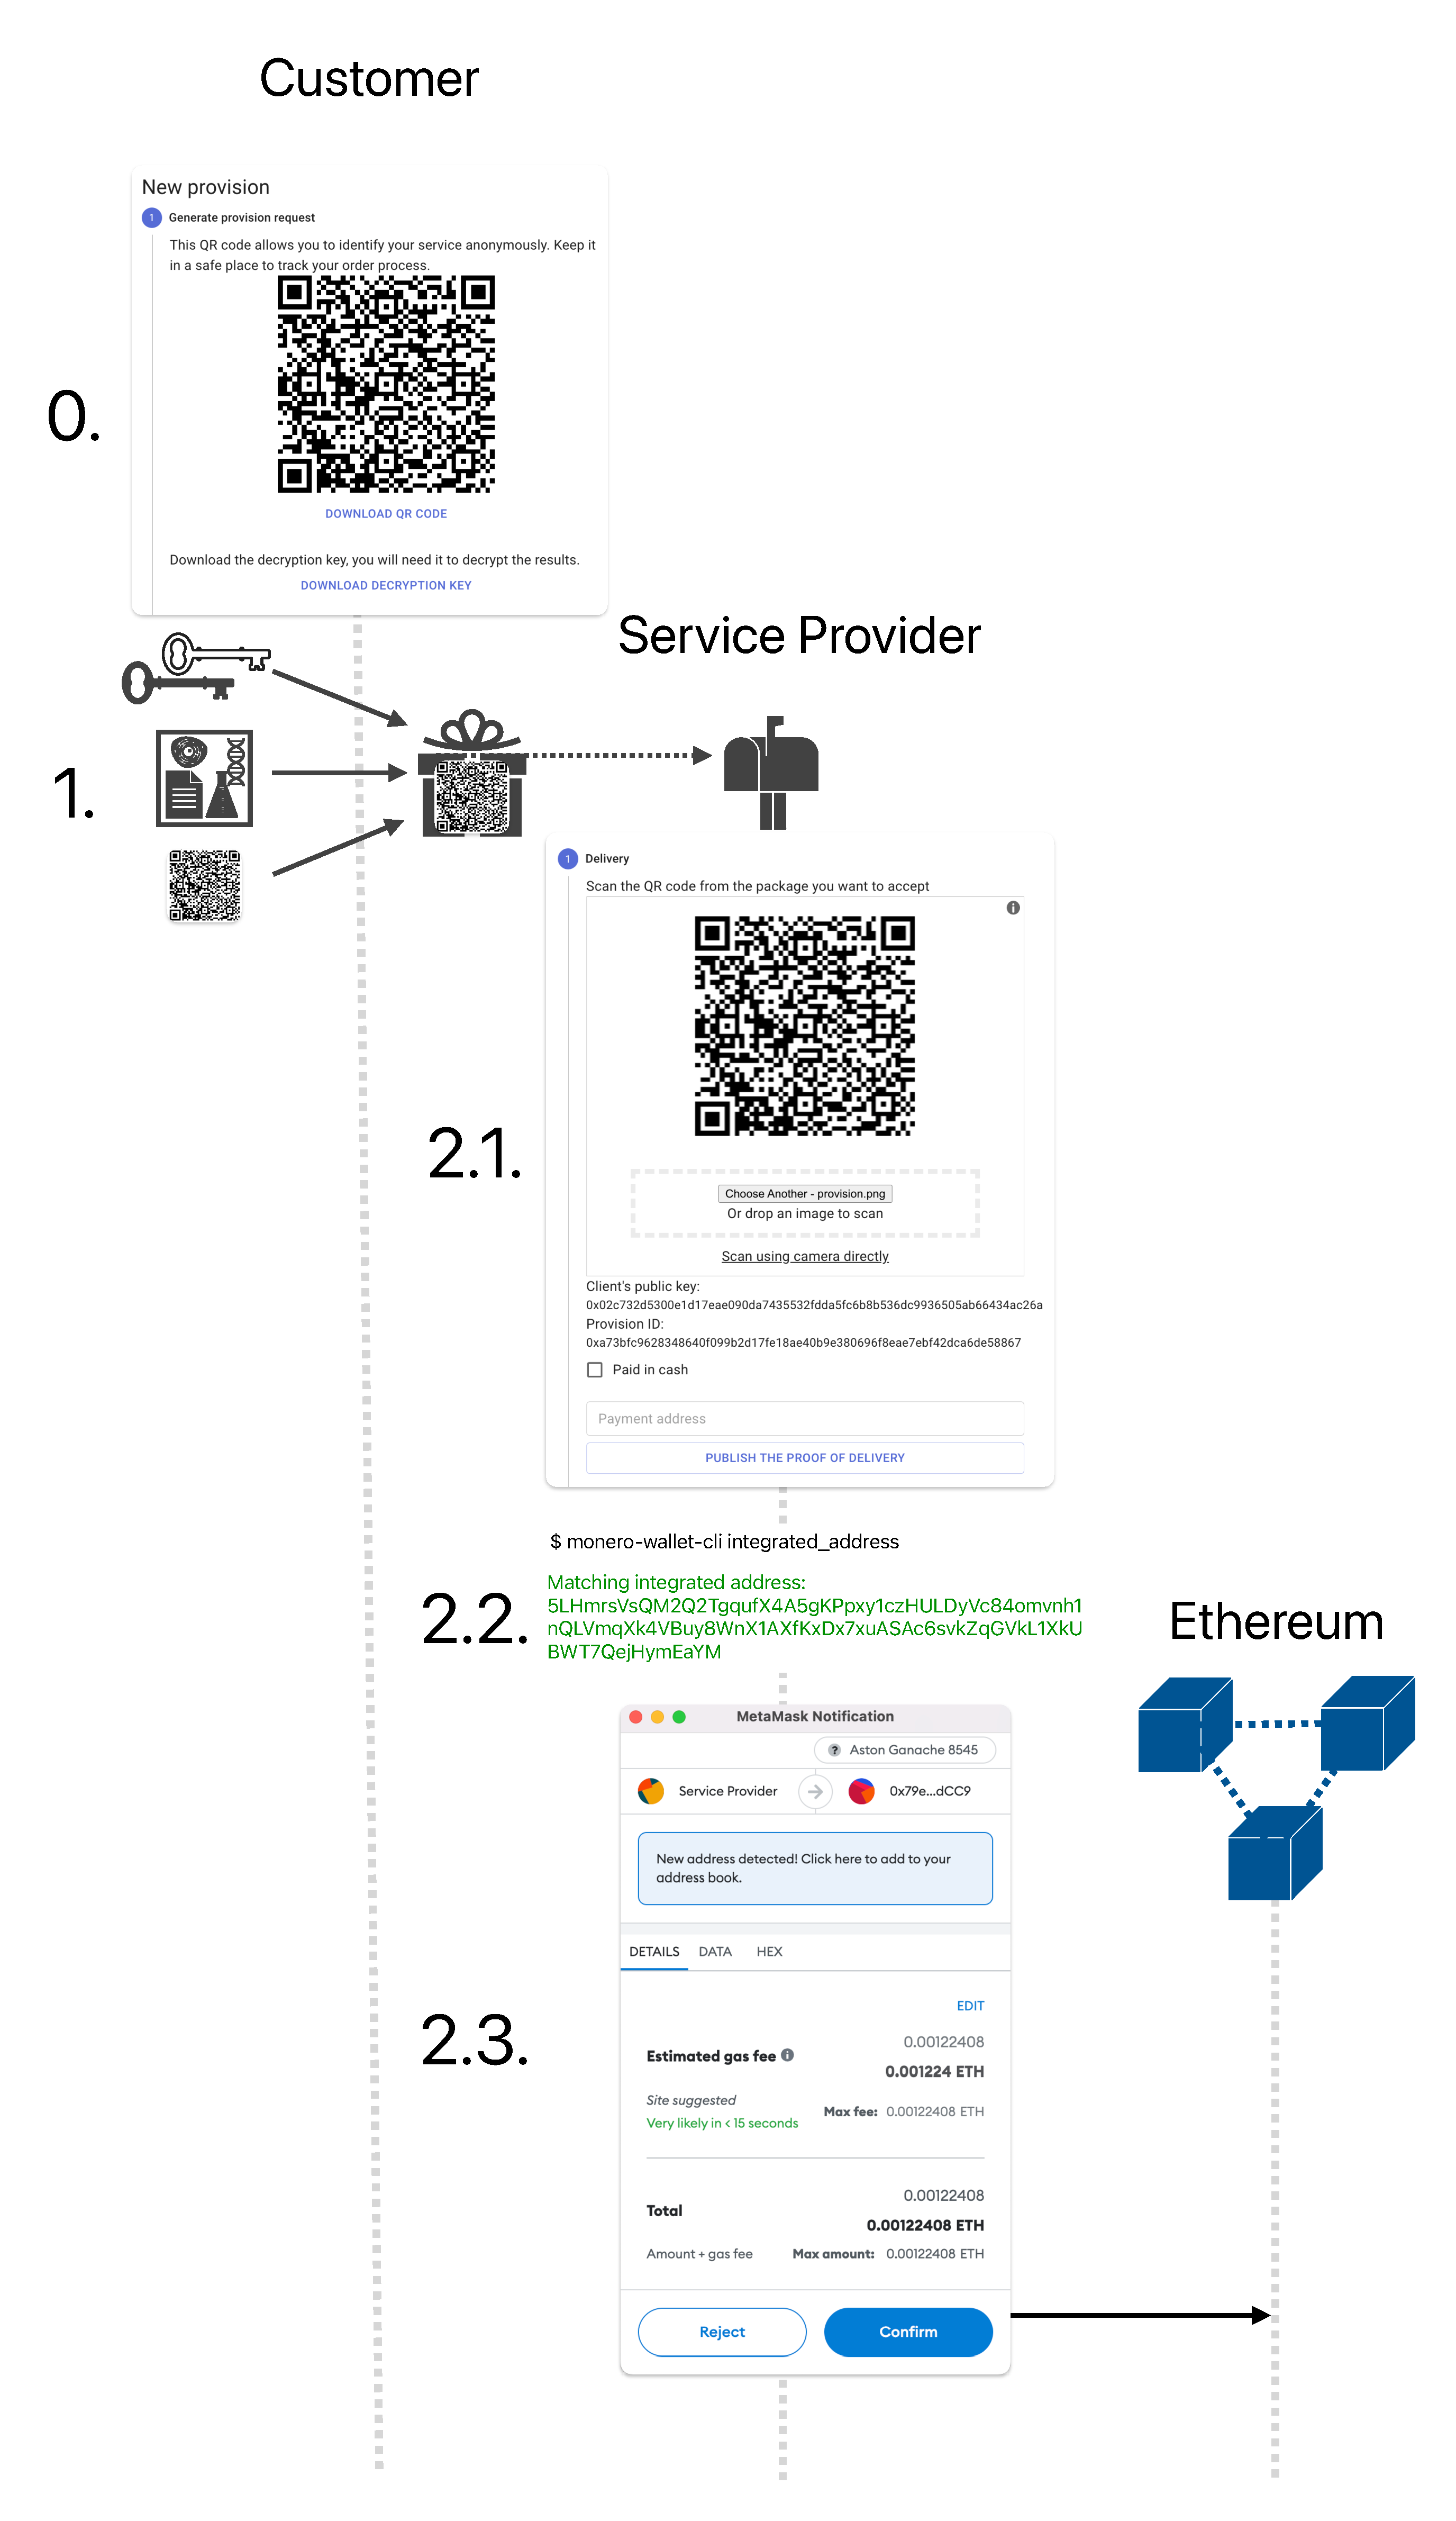
\includegraphics[height=0.95\textheight,keepaspectratio]{anonser-experiment1.pdf}}
\captionof{figure}{Steps of the experiment, first part.}\label{fig:anonser-experiment1}
\end{minipage}

\noindent%
\begin{minipage}{\linewidth}
\makebox[\linewidth]{
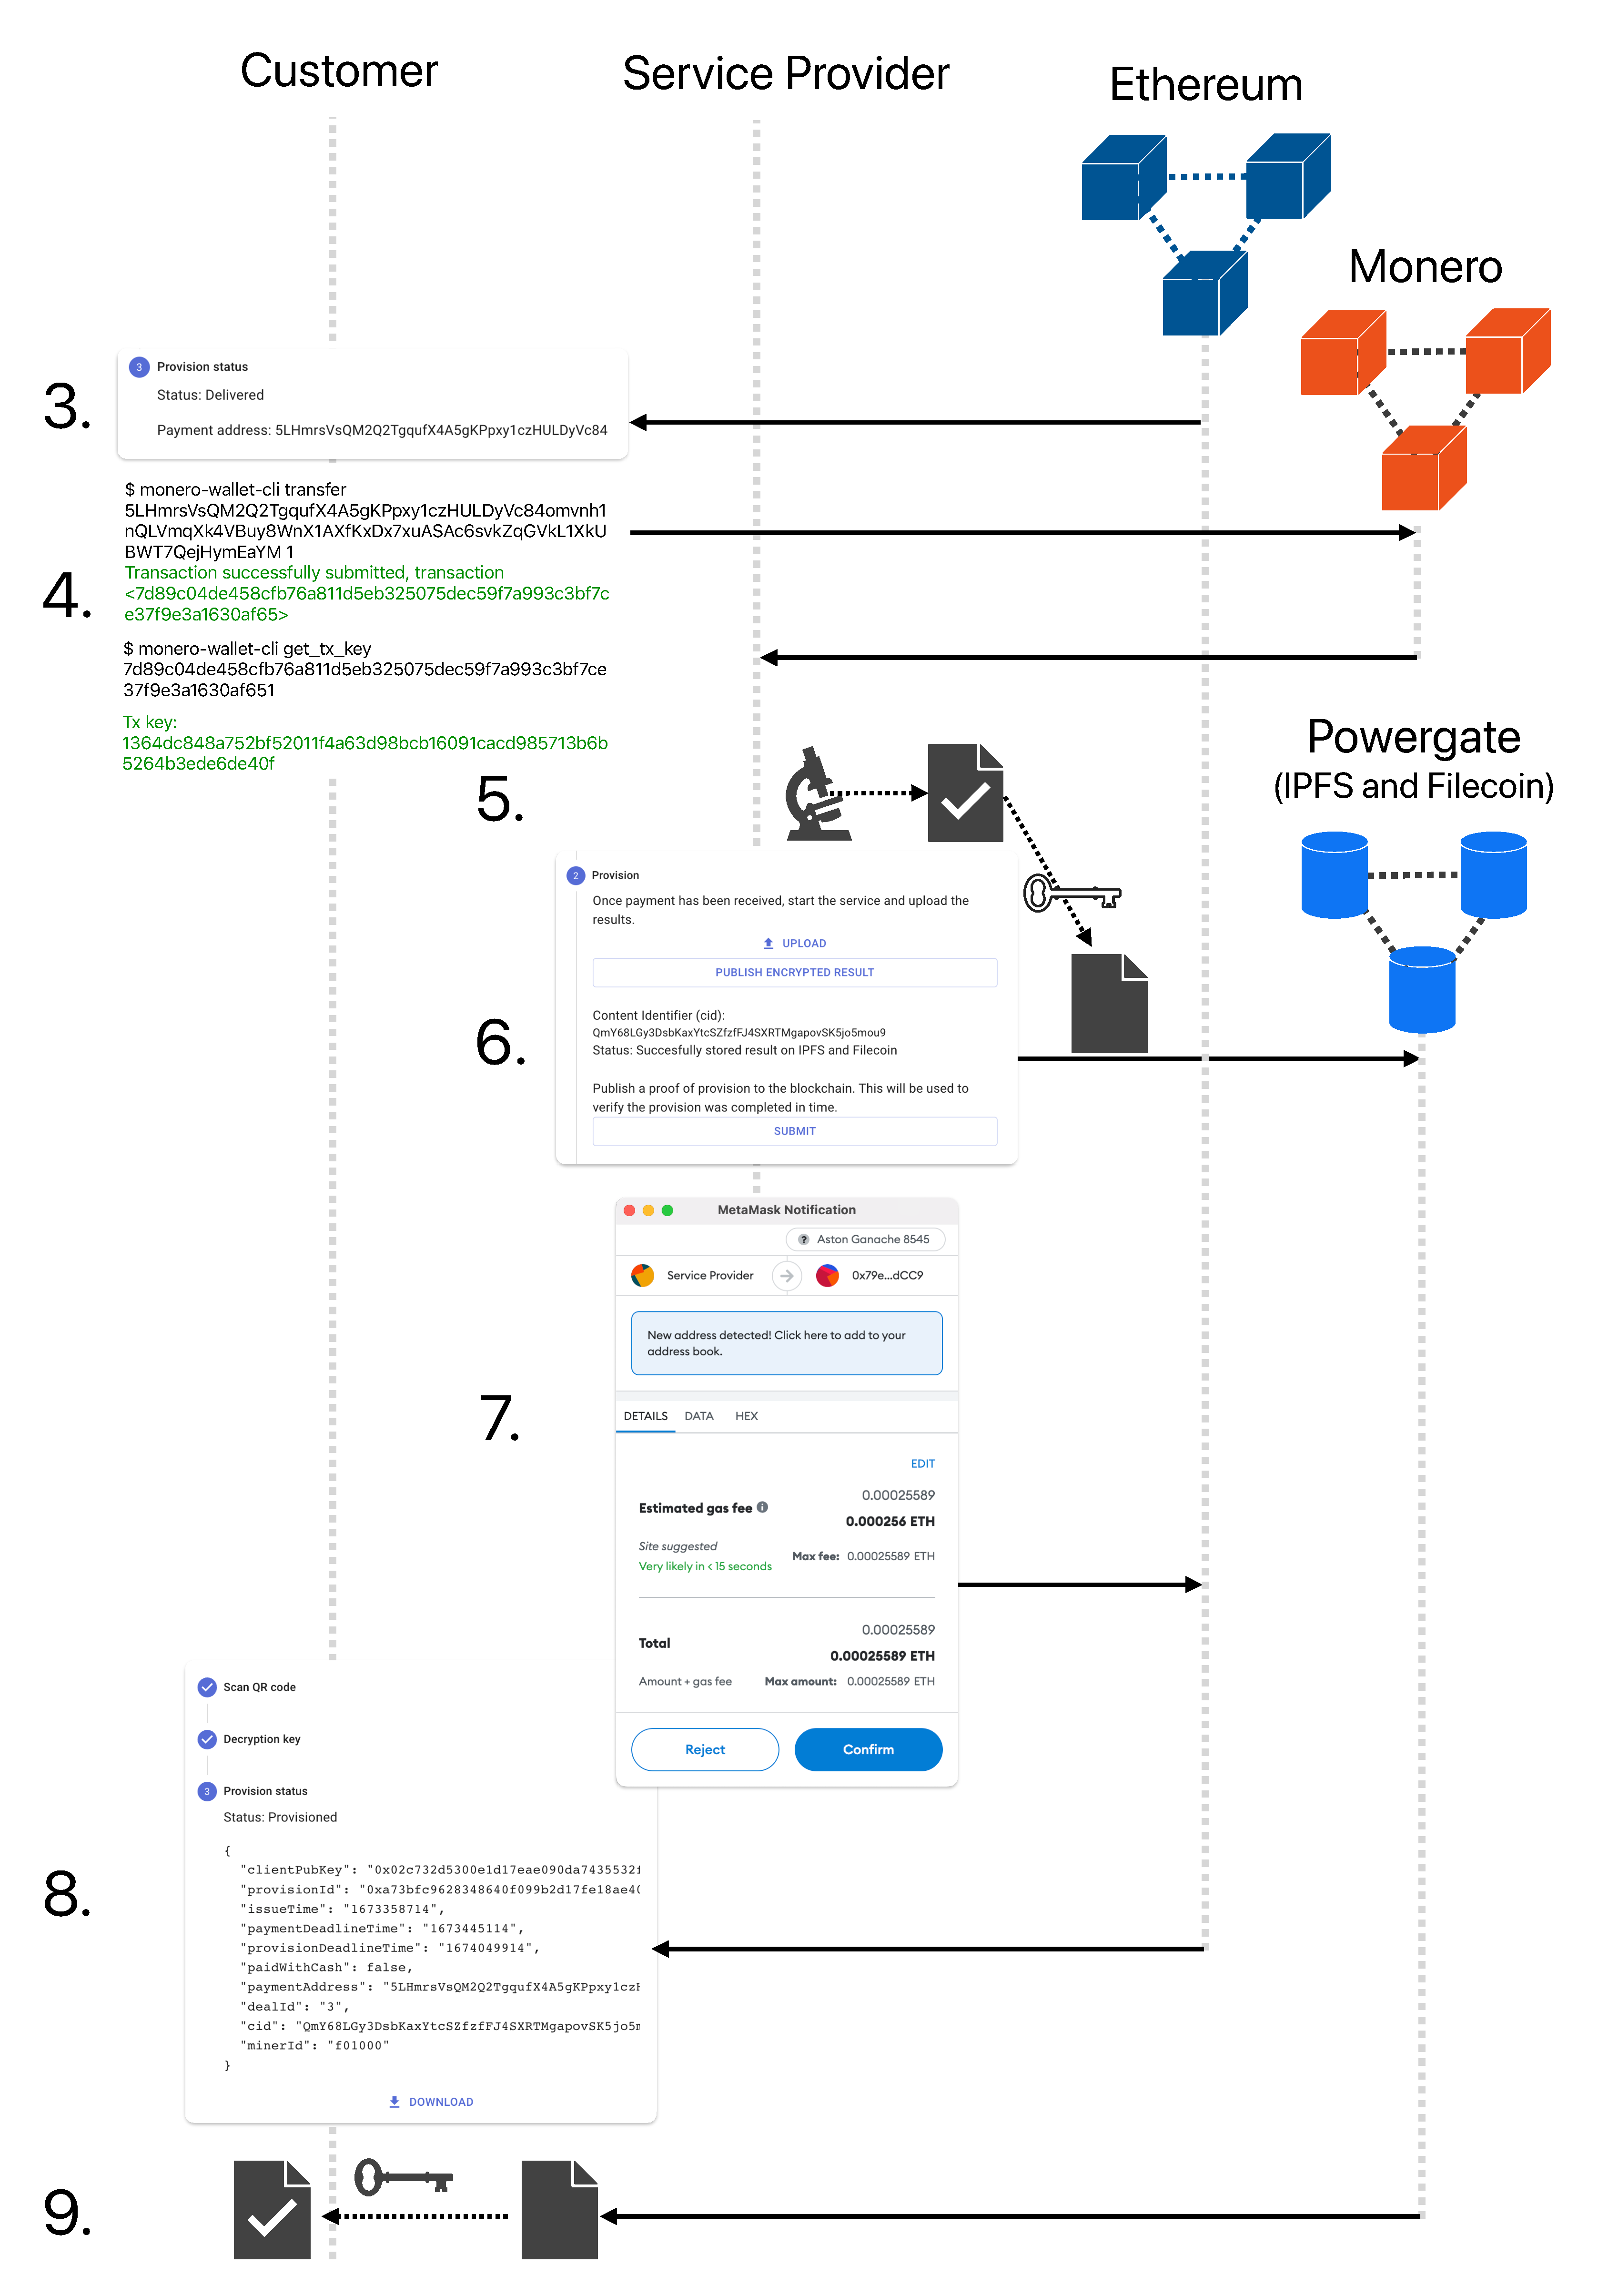
\includegraphics[height=0.95\textheight,keepaspectratio]{anonser-experiment2.pdf}}
\captionof{figure}{Steps of the experiment, second part.}\label{fig:anonser-experiment2}
\end{minipage}
\else
\begin{figure*}
  \centering
  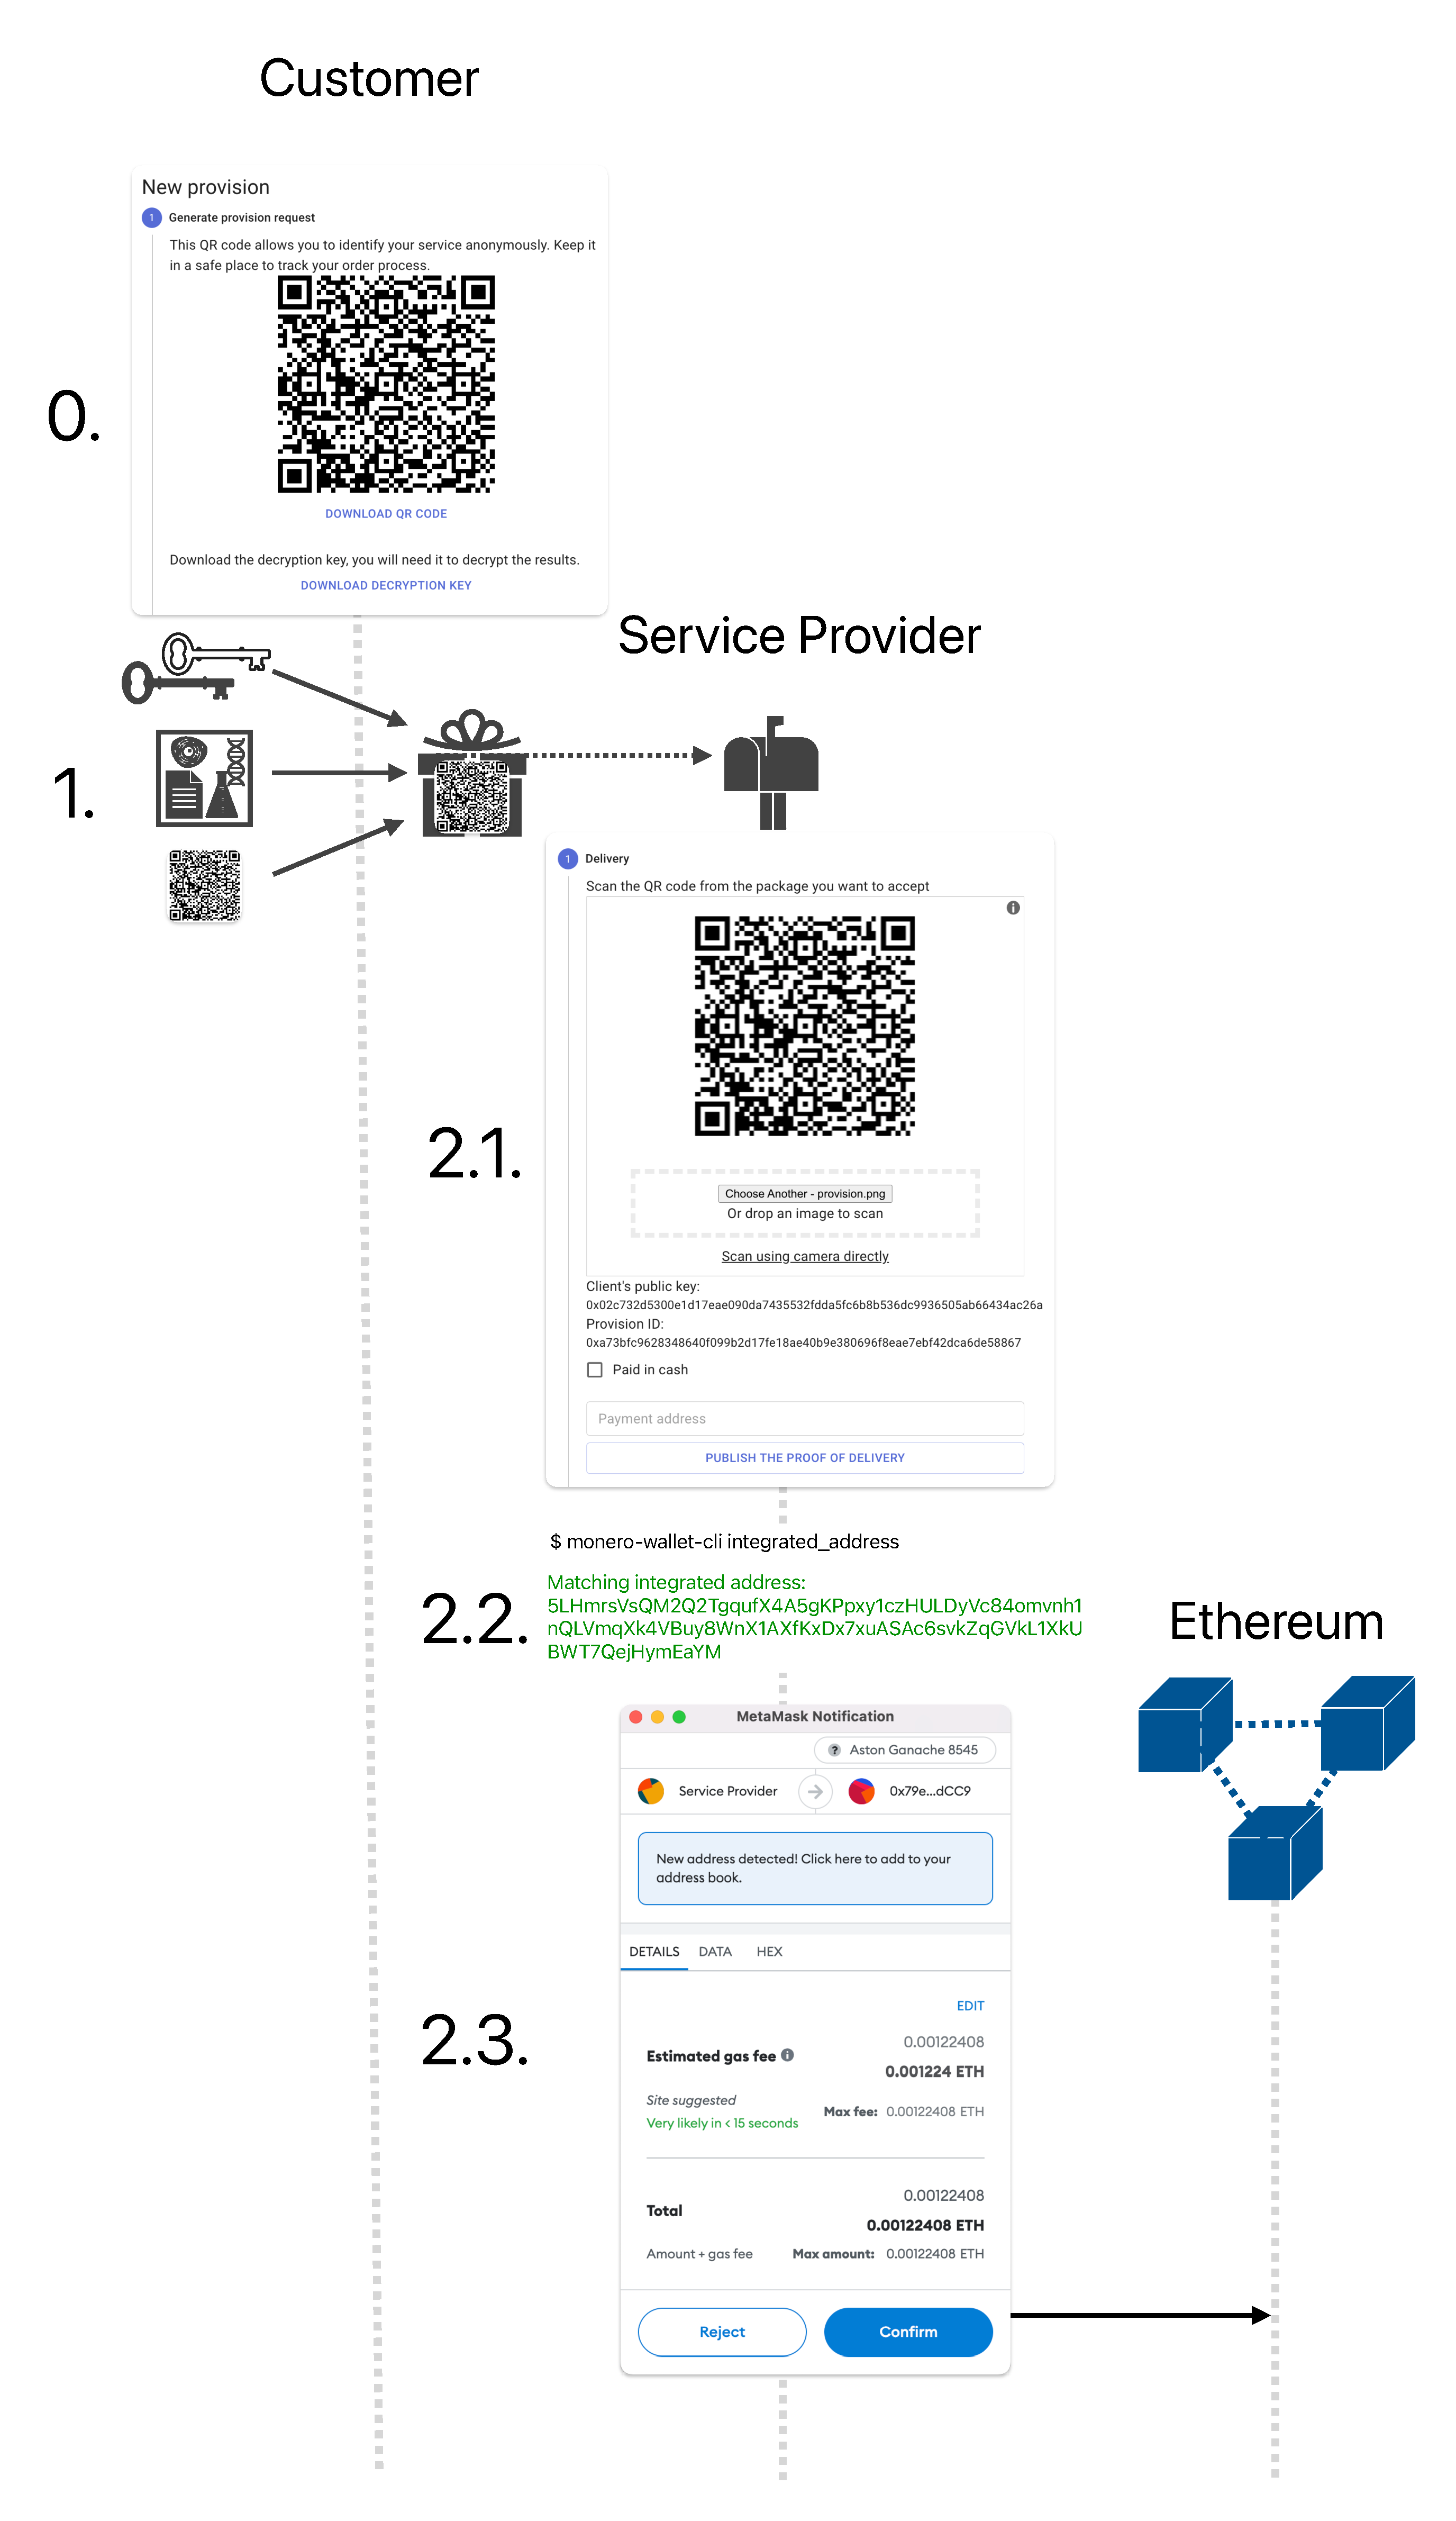
\includegraphics[height=0.95\textheight,keepaspectratio]{anonser-experiment1.pdf}
  \caption{Steps of the experiment, first part.}\label{fig:anonser-experiment1}
\end{figure*}

\begin{figure*}
  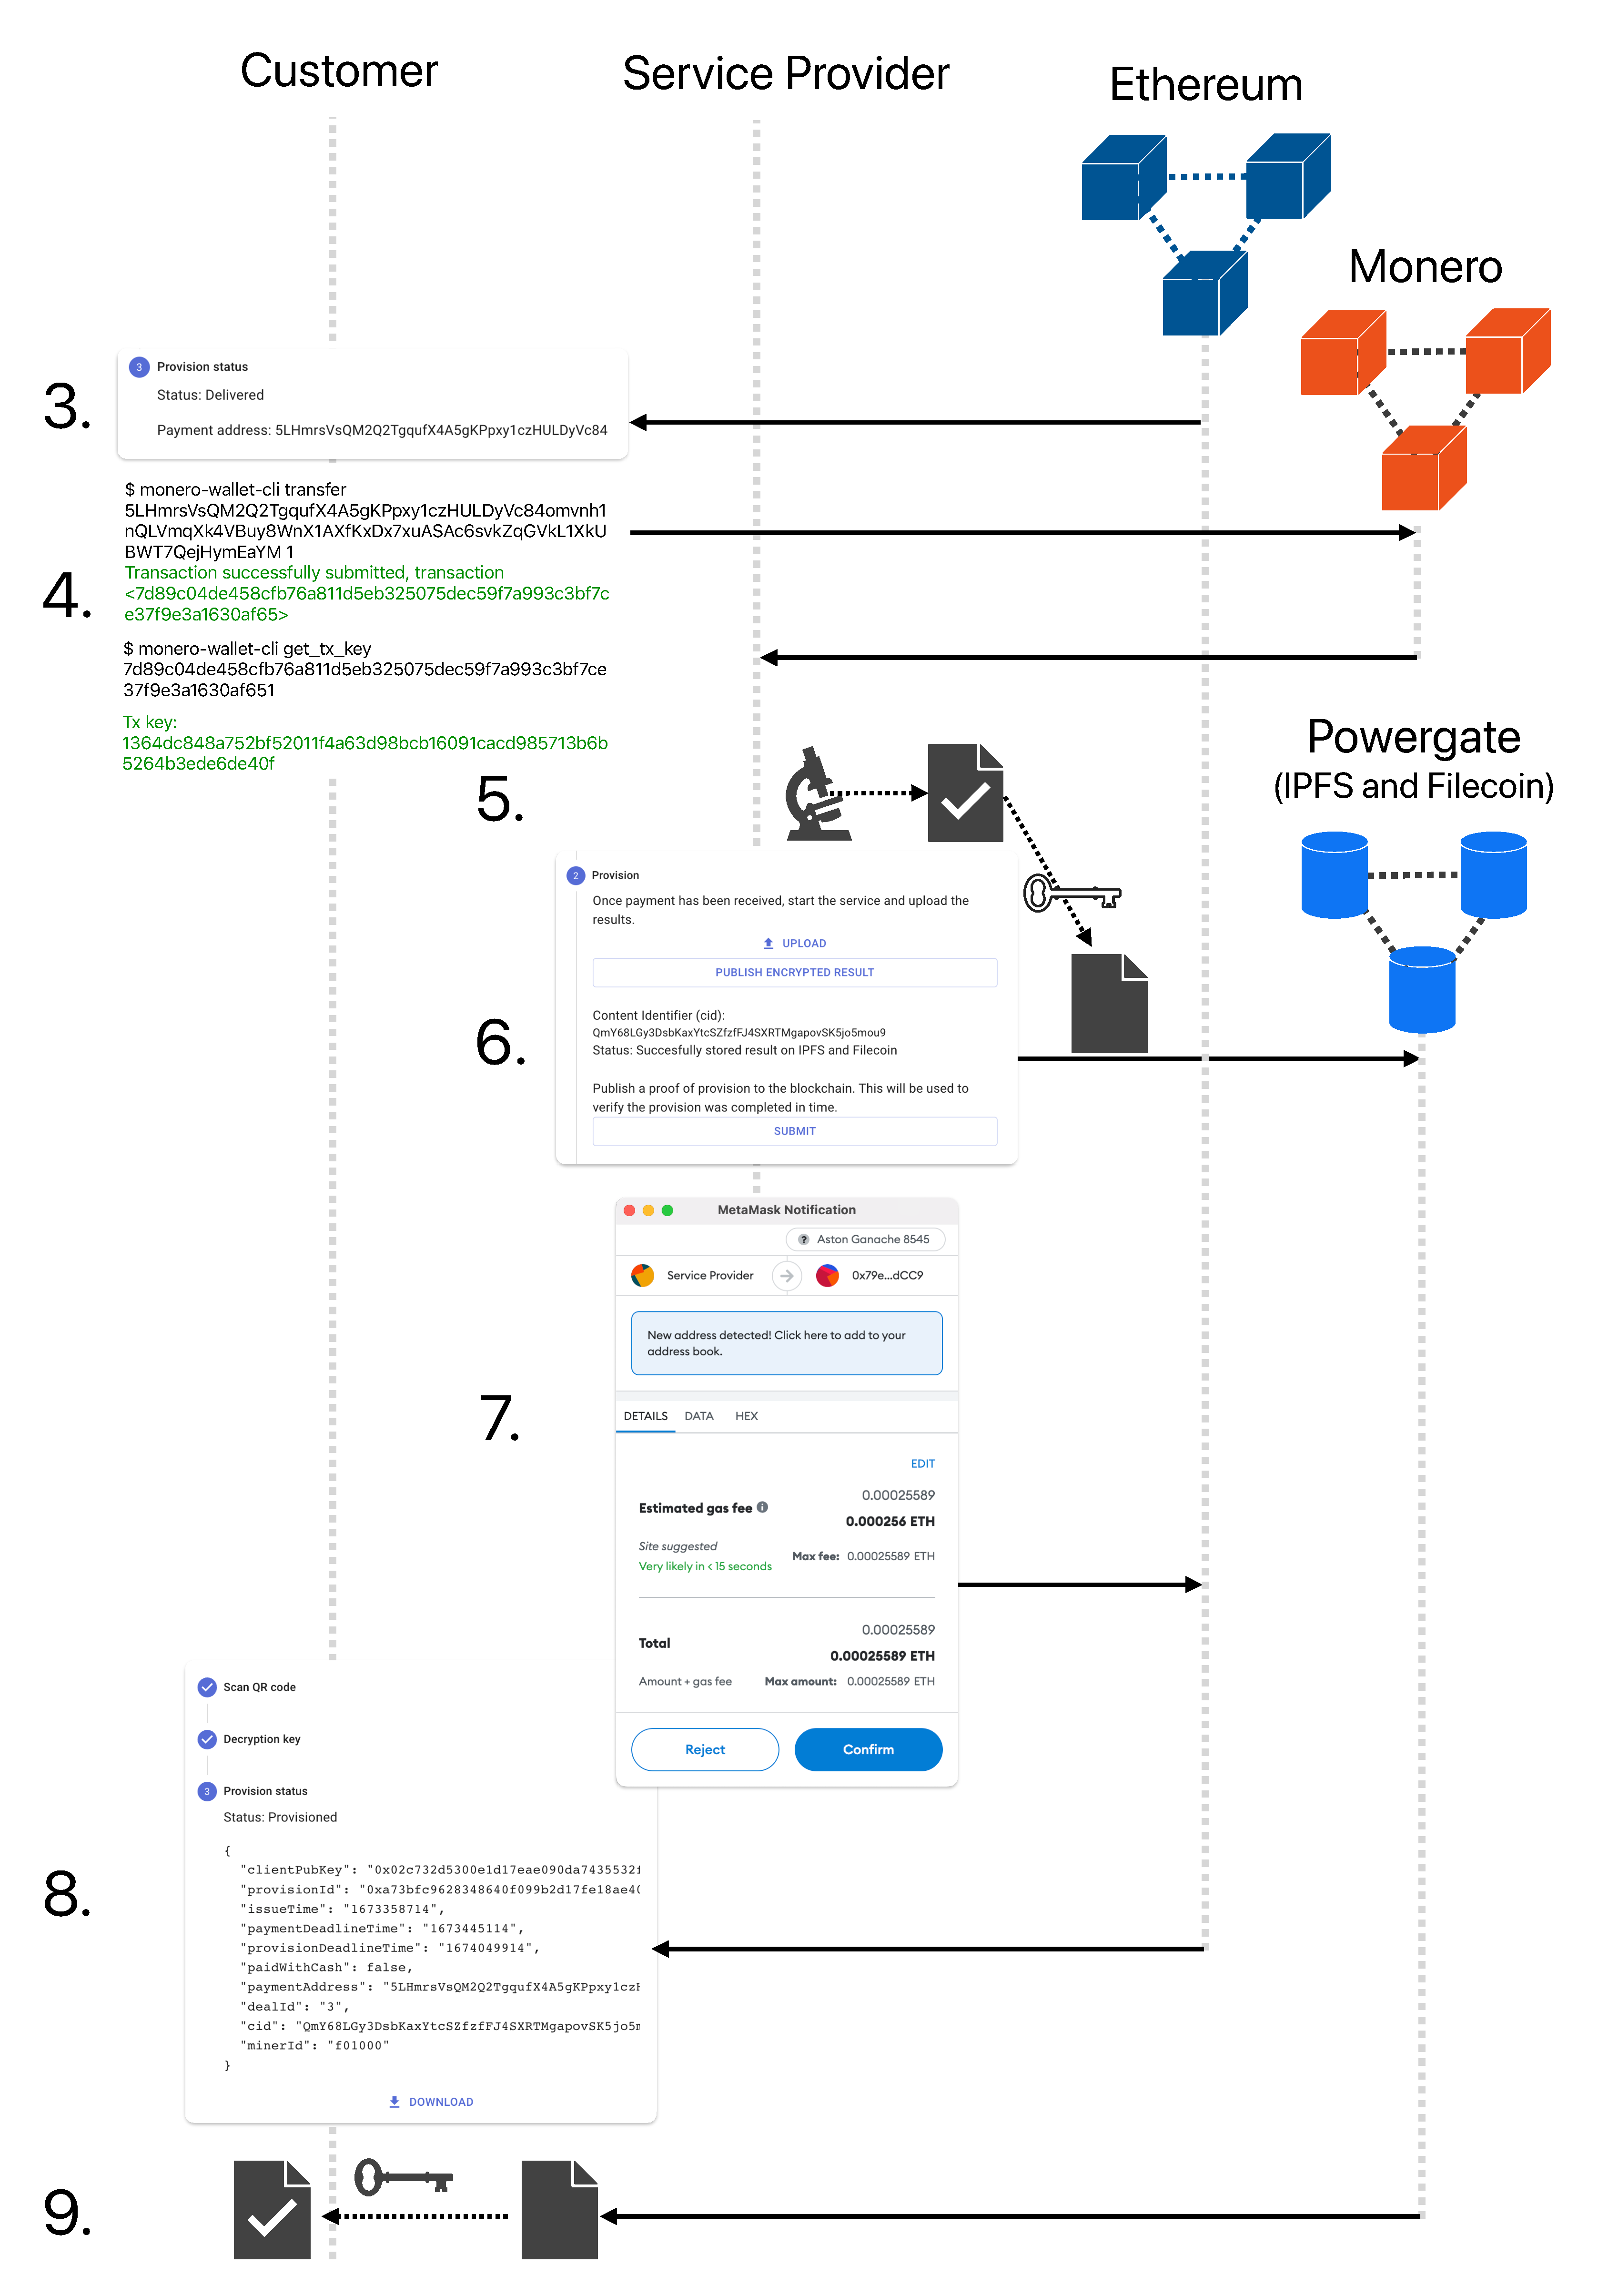
\includegraphics[height=0.95\textheight,keepaspectratio]{anonser-experiment2.pdf}
  \caption{Steps of the experiment, second part.}\label{fig:anonser-experiment2}
\end{figure*}

\fi
\subsection{Results}

\paragraph{Fariness}
As shown in Section~\ref{sec:steps} and~\ref{app:proof-of-fairness}, 
the protocol is fair. It is achieved by an undeniable hand-shake mechanism in which the SP first publishes $\mathrm{PoD}$ (step 2.) committing to package delivery and deadlines of the service, and then the customer accepts it by paying for the service or not (step 3.).

Once the payment is made, the SP stays in the advantaged position. Since he has agreed on the deadlines of the provision of the service, he is incentivized
to provide the service and publish the results and PoP before the deadline (step 7.); otherwise the customer—having all the evidence—can initiate a dispute and punish the SP, therefore rational parties will follow the protocol.

Non-repudiation without TTP is achieved by using the blockchain and digital signatures. Blockchain guarantees that each change to the state of the smart contract is visible to everyone and only the SP is allowed to modify its state. 

\paragraph{Anonymity}
We achieved anonymity by using anonymous payment methods such as cash or privacy-preserving payment blockchains (e.g., Monero), and decentralized storage networks like IPFS and Filecoin, allowing the customer to interact with the protocol without revealing his identity at any step of the protocol.

\paragraph{Provable Results Availability}
Content addressable networks such as IPFS can not guarantee the availability of the content\footnote{Nothing prevents the SP from publishing the result, receiving the $\mathrm{cid}$, publishing $\mathrm{PoP}$, and immediately after removing the result from the local storage. In case of dispute, the SP can upload the content again, proving its availability. The SP has no motivation to proceed with this kind of misbehavior other than putting the customer in a disadvantaged position caused by the lost dispute.}. However, the Filecoin~\cite{protocollabsFilecoinDecentralizedStorage2017}, which works as an incentivization layer on top of IPFS, increases the content availability via economic incentivisation (i.e., punishment in case of lack of proof of storage of the content~\cite{filecoinSlashing}). Compared to typical blockchain networks, Filecoin focuses on data storage and thus makes it cheaper than storing it on blockchains like Bitcoin or Ethereum.

The SP uploads the result on both IPFS and Filecoin networks (via Powergate) making the result free in case of normal behaviour, and highly-available in case of the SP stops serving the result from his node. 

\paragraph{Costs}
Deploying a smart contract and invoking functions on the Ethereum blockchain costs gas. The cost of gas is proportional to the amount of computation required to execute a transaction. 

Deploying a smart contract consumed 1456577 gas.
Proof of delivery consumed 129649 gas.
Proof of provision consumed 149130 gas.

Although our experiment was conducted on testnet, the amount of gas is the same on mainnet.

The cost of gas is denominated in $\mathrm{ETH}$. The price of gas at the time of the experiment (Jan. 03, 2023, \url{https://etherscan.io/gastracker}) was $0.000000002227 \frac{\mathrm{ETH}}{\mathrm gas}$, and the price of 1 $\mathrm{ETH}$ was $1261.97 \mathrm{USD}$.

In a result, the cost of:
\begin{itemize}
  \item Deploying the smart contract cost $0.000000002227 \frac{\mathrm{ETH}}{\mathrm gas} \cdot 1456577 \mathrm{gas} \cdot 1261.97 \frac{\mathrm{USD}}{\mathrm{ETH}} \approx 4.09 \mathrm{USD}$; 
  \item Proof of delivery cost $0.000000002227 \mathrm{\frac{ETH}{gas}} \cdot 129649 \mathrm{gas} \cdot 1261.97 \frac{\mathrm{USD}}{\mathrm{ETH}} \approx 0.29 \mathrm{USD}$; 
  \item Proof of provision cost $0.000000002227 \mathrm{\frac{ETH}{gas}} \cdot 149130 \mathrm{gas} \cdot 1261.97 \frac{\mathrm{USD}}{\mathrm{ETH}} \approx 0.33 \mathrm{USD}$.
\end{itemize}


\section{Discussion}
\label{sec:discussion}

\subsection{Justice}\label{sec:decentralised-justice}

Centralized justice is the biggest obstacle in achieving a system that complies with Web3 postulates~\cite{ethereumWhatWeb3Why2023}.

The possible directions for mitigation of such issues are to either (i) replace local justice with blockchain dispute resolution systems like those proposed in Themis~\cite{mengThemisDecentralizedEscrow2019}, Kleros~\cite{bergollaKlerosSociolegalCase2022,gudkovCrowdArbitrationBlockchain2020}, Aragon Court~\cite{aragonDecentralizedDisputeResolution}, LTO Network~\cite{ltonetworkNextGenBlockchainB2B}, and other Online Dispute Resolution platforms~\cite{allenGovernanceBlockchainDispute2019}; or (ii) make it infeasible to provide incorrect results.

The first approach is more feasible in the near future. It would require creating a large set of experts in a field that, in case of dispute, would receive all the proofs ($\mathrm{PoD}$, $\mathrm{PoP}$, payment $\mathrm{receipt}$ as well as any other proofs significant to the case) that could be queried by the experts in zero-knowledge fashion, i.e., they could ask a limited number of questions to the proofs and getting yes/no answers. The case would be fully confidential as they would not be able to query personal information. The experts would be incentivized to participate in the pool by the system of fees. They would be incentivized to vote honestly by the stake they would have to lock and reward/punishment they would get by judging correctly/incorrectly, where the correctness is determined by the quorum of votes.

The second approach is more futuristic. Suppose that the service we are undertaking is fully computable. Then, it would be possible by employing proofs of correctness of computations~\cite{ben-sassonSNARKsVerifyingProgram2013} to enforce that only correct computations (hence correct services) are accepted. It would require the complete service examination to be computable, which is hard to achieve in settings where physical materials (like blood) are examined. Concretely, the problem canes down to ``How to represent blood digitally?''. If we could represent urine, blood, saliva, or any other physical material in a binary format and let the customer take a sample, discrete it, and send it to the SP, then the whole chain of integrity could be ensured. Therefore, incorrect service provision would be infeasible, and hence, disputes would be avoided.

\subsection{Self-sovereign identities}
Our research in the field showed that some jurisdictions require SPs to associate the diagnosis with the customer's personal information. For example, in Poland, all laboratories performing medical diagnostic tests, and collecting the material (except tests for HIV) are obligated to the unambiguous identification and verification of the identity of the patient from whom the material was collected~\cite{ministerstwozdrowiaRegulationMinisterHealth2006}.

This conflicts with the main goal of our protocol, which is to prevent any identification information from being collected.

One promising solution would be to use Self-sovereign identities (SSI)~\cite{muhleSurveyEssentialComponents2018}, especially the verifiable claims. A trusted authority (e.g., a government) would issue a one-time claim for a customer that would be accepted by the SP as legitimate personal identification. The SP would associate the diagnosis result with the provided DID. The DID itself would not contain any personal information, therefore the SP would learn nothing about the customer's identity besides the random-looking identification. The DID could be deanonimised by collaboration with the government.

However, since SSI is a relatively new technology and the government has not yet adopted it, we decided to postpone the discussion of this topic to future work.

\subsection{Formal Verification}\label{sec:formal-verification}
Following the work of~\cite{birjoveanuFormalVerificationMultiparty2022}, the security analysis of our protocol could be improved by the usage of tools for the automatic formal verification, e.g., AVISPA~\cite{armandoAVISPAToolAutomated2005}. It would require specifying the protocol using High-Level Protocol Specification Language (HLPSL)~\cite{chevalierHighLevelProtocol2004}. The specification would be then translated to the AVISPA's intermediate language and verified using the AVISPA's theorem prover. The verification would be performed by the AVISPA's model checker, which would check the protocol against the security properties.

\section{Conclusions}\label{sec:conclusion}
In this work, we have focused on enabling service provision without the collection of personal data. Our aim was to enable services such as genetic tests, tests for paternity, venereal diseases, HIV, drugs, and steroids, or anonymous legal advice.

We observed that the current state of the art is not sufficient to achieve the goal. Therefore, we have proposed a protocol for service provision that simultaneously achieves anonymity, fairness, dispute resolution, TTP-lessness, and supports physical materials.

Payments are handled either in cash or anonymous cryptocurrencies. The result of the service is published on a content-addressable p2p network. The dispute can be settled by disclosing the collected proofs to justice. 

Using the definition~\ref{def:fairness} we showed that the protocol achieves fairness by the proof of delivery, payment receipt, and proof of provision published on the message board. 

Finally, we pinpointed further improvements like decentralized dispute resolution, self-sovereign identifiers, and anonymous package delivery via courier.

\appendix

\section{Proof of fairness}\label{app:proof-of-fairness}
Below we describe each step and rationale of the outcome position.
We use the notation introduced in Section~\ref{sec:fairness-model} to analyze each position in the protocol and fairness Definition~\ref{def:fairness} to show the fairness of the protocol.

\newcommand{\AgreeablePath}{Agreeable path:}
\newcommand{\DisputePath}{The \customer{} starts a dispute:}
\newcommand{\Fairness}{Fairness:}
\newcommand{\CustomerTurn}[0]{\expandafter\MakeUppercase \customer{} turn:}
\newcommand{\SPTurn}[0]{\sp{} turn:}

\newcommand{\CanFollowToOne}[2]{The #1 can follow the protocol to the non-disadvantaged position #2}
\newcommand{\CanDoNothing}[1]{The #1 can do nothing and always ends up in the non-disadvantaged position}
\newcommand{\CanDoAnything}[1]{The #1 can do anything and always ends up in the non-disadvantaged position}
\newcommand{\Pos}[4]{$\operatorname{\sigma_{#1, #2, #3} = #4}$}
\newcommand{\WinForTheSameReason}[1]{The #1 wins the dispute for the same reason}
\newcommand{\LoseForTheSameReason}[1]{The #1 loses the dispute for the same reason}
\newcommand{\ActedAbnormallyThen}[1]{The #1 acted abnormally, then:}
\newcommand{\CustomerPaidButDidntGetResult}{the customer ends up in a disadvantaged position as he paid in advance but didn't receive the result}
\newcommand{\SpReceivedThePayment}{the SP ends up in the advantaged position as she received the payment}

\newcommand{\CustomerLosesBeforePayment}{The customer loses the dispute because the SP is not obligated to do anything until the transaction is paid}
\newcommand{\CustomerLosesBeforePoP}{The customer loses the dispute because the SP still can publish the PoP within the agreed timeframe}

\newcommand{\RemainsIn}[2]{The #1 remains in the #2 position}

\subsubsection*{Step 1. \CustomerTurn{} Package delivery}\label{step-1-deliver-package}

The protocol starts when the customer correctly executes the first step of the protocol, i.e., deliver the package to the SP. 

The case where the customer does not deliver the package is not considered as it is not a part of the protocol.

\begin{itemize}
\item \AgreeablePath
  \begin{itemize}
    \item  \Pos{1}{c}{\normal}{\neutral}, the customer risked his materials but did not pay for the transaction and therefore ends up in a neutral position (see Assumption 10. in Section \ref{sec:assumptions}).
    \item \Pos{1}{s}{\normal}{\neutral}, the SP ends up in a neutral position as she did not spend any resources and the package did not bring her any value.
  \end{itemize}
\item \DisputePath
  \begin{itemize}
    \item \Pos{1}{c}{\dispute}{\minus}, \CustomerLosesBeforePayment{}.
    \item \Pos{1}{s}{\dispute}{\neutral}, \WinForTheSameReason{SP}.
  \end{itemize}
\end{itemize}

\Fairness

\begin{itemize}
  \item \CanFollowToOne{customer}{\Pos{1}{c}{n}{\neutral}}
  \item \CanDoNothing{SP}
\end{itemize}

\subsubsection*{Step 2. \SPTurn{} Proof of Delivery}\label{step-2-proof-of-delivery}

The SP publishes the PoD, then:

\begin{itemize}
  \item \AgreeablePath
    \begin{itemize}
      \item \Pos{2}{c}{\normal}{\neutral}, the customer remains in the neutral position as the PoD allows him to pay for the transaction but does not obligate him to anything.
      \item \Pos{2}{s}{\normal}{\neutral}, the SP remains in the neutral position as the package has not brought her any value and she did not spend any resources to provide the service yet.
    \end{itemize}

  \item \DisputePath
    \begin{itemize}
      \item \Pos{2}{c}{\dispute}{\minus}, \CustomerLosesBeforePayment{}.
      \item \Pos{2}{s}{\dispute}{\neutral}, \WinForTheSameReason{SP}.
    \end{itemize}
\end{itemize}

\ActedAbnormallyThen{\sp}

\begin{itemize}
\item \AgreeablePath
  \begin{itemize}
    \item \Pos{2}{c}{\abnormal}{\neutral}, the customer remains in the neutral position as he is not obligated\footnote{By not obligated we understand the situation where a party does not risk any resources by not taking the action} to agree with the incorrect $\mathrm{PoD}$.
    \item \Pos{2}{s}{\abnormal}{\neutral}, the SP remains in the neutral position as the package has not brought her any value and she did not spend any resources to provide the service yet.
  \end{itemize}
\item \DisputePath
  \begin{itemize}
    \item \Pos{2}{c}{\abdispute}{\minus}, \CustomerLosesBeforePayment{}, not even to publish correct $\mathrm{PoD}$.
    \item \Pos{2}{s}{\abdispute}{\neutral}, \WinForTheSameReason{SP}.
  \end{itemize}
\end{itemize}

\Fairness

\begin{itemize}
  \item \CanDoAnything{SP}.
  \item The customer can either wait (in case of the SP following the protocol) or abandon the transaction (in case of the SP acting abnormally). In both cases the customer ends up in non-disadvantaged position \Pos{2}{c}{\normal}{\neutral} or \Pos{2}{c}{\abnormal}{\neutral}.
\end{itemize}


\subsubsection*{Step 3. \CustomerTurn{} Get Proof of Delivery}\label{step-3-get-proof-of-delivery}

The customer got the \PoD, then:

\begin{itemize}
\item \AgreeablePath
  \begin{itemize}
    \item \Pos{3}{c}{\normal}{\neutral}, \RemainsIn{customer}{neutral}.
    \item \Pos{3}{s}{\normal}{\neutral}, \RemainsIn{SP}{neutral}.
  \end{itemize}
\item \DisputePath
  \begin{itemize}
    \item \Pos{3}{c}{\dispute}{\minus}, \CustomerLosesBeforePayment{}.
    \item \Pos{3}{s}{\dispute}{\neutral}, \WinForTheSameReason{SP}.
  \end{itemize}
\end{itemize}

\ActedAbnormallyThen{\customer}

\begin{itemize}
\item \AgreeablePath
  \begin{itemize}
    \item \Pos{3}{c}{\abnormal}{\neutral}, \RemainsIn{customer}{neutral}.
    \item \Pos{3}{s}{\abnormal}{\neutral}, \RemainsIn{SP}{neutral}.
  \end{itemize}
\item \DisputePath
  \begin{itemize}
    \item \Pos{3}{c}{\abdispute}{\minus}, \CustomerLosesBeforePayment{}.
    \item \Pos{3}{s}{\abdispute}{\neutral}, \WinForTheSameReason{SP}.
  \end{itemize}
\end{itemize}

\Fairness

\begin{itemize}
  \item \CanFollowToOne{customer}{\Pos{3}{c}{\normal}{\neutral}}.
  \item \CanDoNothing{SP}.
\end{itemize}



\subsubsection*{Step 4. \CustomerTurn{} Payment}

The customer paid the transaction, then:

\begin{itemize}
\item \AgreeablePath
  \begin{itemize}
    \item \Pos{4}{c}{\normal}{\minus}, the customer paid in advance.
    \item \Pos{4}{s}{\normal}{\plus}, the SP received the payment but has not spent his resources yet.
  \end{itemize}
\item \DisputePath
  \begin{itemize}
    \item \Pos{4}{c}{\dispute}{\minus}, \CustomerLosesBeforePoP{}.
    \item \Pos{4}{s}{\dispute}{\neutral}, \WinForTheSameReason{SP}.
  \end{itemize}
\end{itemize}

\ActedAbnormallyThen{\customer}

\begin{itemize}
\item \AgreeablePath
  \begin{itemize}
    \item \Pos{4}{c}{\abnormal}{\neutral}, the customer ends up in the neutral position as he did not spend his funds.
    \item \Pos{4}{s}{\abnormal}{\neutral}, the SP ends up in the neutral position as she neither received the payment nor spent her resources.
  \end{itemize}
\item \DisputePath
  \begin{itemize}
    \item \Pos{4}{c}{\abdispute}{\minus}, \CustomerLosesBeforePayment{}.
    \item \Pos{4}{s}{\abdispute}{\neutral}, \WinForTheSameReason{SP}.
  \end{itemize}
\end{itemize}

\Fairness

\newcommand{\CustomerRiskTemporaryDisadvantagedPosition}[1]{The customer, following the 9th assumption described in Section~\ref{sec:assumptions}, risk the temporary disadvantaged position #1 in favor of a later better position \Pos{9}{s}{\normal}{\plus}; meanwhile being able to get out of the disadvantaged position if the SP misbehave in one of the following steps.}

\begin{itemize}
  \item \CustomerRiskTemporaryDisadvantagedPosition{\Pos{4}{c}{\normal}{\minus}}.
  \item \CanDoNothing{SP}.
\end{itemize}



\subsubsection*{Step 5. \SPTurn{} Provision of service}

The \sp{} did the provision of service, then:

\begin{itemize}
\item \AgreeablePath
  \begin{itemize}
    \item \Pos{5}{c}{\normal}{\minus}, \RemainsIn{\customer}{disadvantaged} as he did not receive the result.
    \item \Pos{5}{s}{\normal}{\plus}, \RemainsIn{\sp}{advantaged} as she received the payment.
  \end{itemize}
\item \DisputePath
  \begin{itemize}
    \item \Pos{5}{c}{\dispute}{\minus}, \CustomerLosesBeforePoP{}.
    \item \Pos{5}{s}{\dispute}{\neutral}, \WinForTheSameReason{SP}.
  \end{itemize}
\end{itemize}

\ActedAbnormallyThen{\sp}

\begin{itemize}
\item \AgreeablePath
  \begin{itemize}
    \item \Pos{5}{c}{\abnormal}{\minus}, \CustomerPaidButDidntGetResult{}. 
    \item \Pos{5}{s}{\abnormal}{\plus}, \SpReceivedThePayment{}.
  \end{itemize}
\item \DisputePath
  \begin{itemize}
    \item \Pos{5}{c}{\abdispute}{\neutral} The customer wins the dispute because the SP did not provide the service within the time agreed upon in the \PoD{}, and so the SP will not be able to upload the result and publish the \PoP{} on time.
    \item \Pos{5}{s}{\abdispute}{\minus}, \LoseForTheSameReason{SP}.
  \end{itemize}
\end{itemize}

\Fairness
\newcommand{\SPCanDoBothButFollowIsSafe}[1]{The SP can follow the protocol and move to the advantaged position \Pos{#1}{s}{\normal}{\plus}, or act abnormally (not provide the service) and also move to the advantaged position \Pos{#1}{s}{\abnormal}{\plus}; however, the second option puts her at risk of terminating the protocol at \Pos{#1}{s}{\abdispute}{\minus} if the customer is rational and starts a dispute; hence, the SP should choose the first option}

\begin{itemize}
  \item \CustomerRiskTemporaryDisadvantagedPosition{\Pos{5}{c}{\normal}{\minus}}.
  \item \SPCanDoBothButFollowIsSafe{5}.
\end{itemize}

\subsubsection*{Step 6. \SPTurn{} Upload result}\label{step-6-publication-of-results}

The SP uploaded the result on time, then:

\begin{itemize}
\item \AgreeablePath
  \begin{itemize}
    \item \Pos{6}{c}{\normal}{\minus}, \RemainsIn{\customer}{disadvantaged} as he did not receive the result.
    \item \Pos{6}{s}{\normal}{\plus}, \RemainsIn{SP}{advantaged} as she received the payment.
  \end{itemize}
\item \DisputePath
  \begin{itemize}
    \item \Pos{6}{c}{\dispute}{\minus}, \CustomerLosesBeforePoP{}.
    \item \Pos{6}{s}{\dispute}{\neutral}, \WinForTheSameReason{SP}.

  \end{itemize}
\end{itemize}

\ActedAbnormallyThen{\sp}

\begin{itemize}
\item \AgreeablePath
  \begin{itemize}
    \item \Pos{6}{c}{\abnormal}{\minus}, \CustomerPaidButDidntGetResult{}.
    \item \Pos{6}{s}{\abnormal}{\plus}, \SpReceivedThePayment{}.
  \end{itemize}
\item \DisputePath
  \begin{itemize}
    \item \Pos{6}{c}{\abdispute}{\neutral}, the customer wins the dispute because the SP did not upload the service within the time agreed upon in the \PoD{}, and so the SP will not be able to publish the \PoP{} on time.
    \item \Pos{6}{s}{\abdispute}{\minus}, \LoseForTheSameReason{SP}.
  \end{itemize}
\end{itemize}

\Fairness

\begin{itemize}
  \item \CustomerRiskTemporaryDisadvantagedPosition{\Pos{6}{c}{\normal}{\minus}}.
  \item \SPCanDoBothButFollowIsSafe{6}.
\end{itemize}

\subsubsection*{Step 7. \SPTurn{} Proof of provision}\label{step-7-publication-of-proof-of-provision}

The SP published \PoP{} on time, then:

\newcommand{\CustomerLosesBecauseSPCanProveBeingCorrect}{the \customer{} loses the dispute as the \sp{} has published all evidences to prove her correct behaviour}

\begin{itemize}
  \item \AgreeablePath
    \begin{itemize}
      \item \Pos{7}{c}{\normal}{\minus}, the customer has not received the result. Therefore, he remains in a disadvantaged position. 
      \item \Pos{7}{s}{\normal}{\plus}, the SP has published all evidence to prove her correct behavior, therefore she remains in an advantaged position for the rest of the protocol.
    \end{itemize}
  \item \DisputePath
    \begin{itemize}
      \item \Pos{7}{c}{\dispute}{\minus}, \CustomerLosesBecauseSPCanProveBeingCorrect{}.
      \item \Pos{7}{s}{\dispute}{\plus}, \WinForTheSameReason{SP}.
    \end{itemize}
\end{itemize}

\ActedAbnormallyThen{\sp}

\begin{itemize}
\item \AgreeablePath
  \begin{itemize}
    \item \Pos{7}{c}{\abnormal}{\minus}, \CustomerPaidButDidntGetResult{}.
    \item \Pos{7}{s}{\abnormal}{\plus}, \SpReceivedThePayment{}.
  \end{itemize}
\item \DisputePath
  \begin{itemize}
    \item \Pos{7}{c}{\abdispute}{\neutral}, the customer wins the dispute because the SP did not publish the correct \PoP{} on time.
    \item \Pos{7}{s}{\abdispute}{\minus}, \LoseForTheSameReason{SP}.
  \end{itemize}
\end{itemize}

\Fairness

\begin{itemize}
  \item \CustomerRiskTemporaryDisadvantagedPosition{\Pos{7}{c}{\normal}{\minus}}.
  \item \SPCanDoBothButFollowIsSafe{7}.
\end{itemize}


\subsubsection*{Step 8. \CustomerTurn{} Get Proof of Provision}\label{step-8-pull-proof-of-provision}

The customer got the \PoP{}, then:

\begin{itemize}
\item \AgreeablePath
  \begin{itemize}
    \item \Pos{8}{c}{\normal}{\minus}, the customer gets the \cid{}, but not the result yet.
    \item \Pos{8}{s}{\normal}{\plus}, \RemainsIn{\sp}{advantaged}.
  \end{itemize}
\item \DisputePath

  \begin{itemize}
    \item \Pos{8}{c}{\dispute}{\minus}, \CustomerLosesBecauseSPCanProveBeingCorrect{}.
    \item \Pos{8}{s}{\dispute}{\plus}, \WinForTheSameReason{SP}.
  \end{itemize}
\end{itemize}

\ActedAbnormallyThen{\customer}

\begin{itemize}
\item \AgreeablePath
  \begin{itemize}
    \item \Pos{8}{c}{\abnormal}{\minus}, the customer paid for the transaction but does not have the access to $cid$, and hence, can not get the result from the storage network.
    \item \Pos{8}{s}{\abnormal}{\plus}, \SpReceivedThePayment{}.
  \end{itemize}
\item \DisputePath
  \begin{itemize}
    \item \Pos{8}{c}{\abdispute}{\minus}, \CustomerLosesBecauseSPCanProveBeingCorrect{}
    \item \Pos{8}{s}{\abdispute}{\neutral}, \WinForTheSameReason{SP}.
  \end{itemize}
\end{itemize}


\Fairness

\begin{itemize}
  \item \CustomerRiskTemporaryDisadvantagedPosition{\Pos{8}{c}{\normal}{\minus}}.
  \item \CanDoNothing{} \Pos{8}{s}{\normal}{\plus} or \Pos{8}{s}{\abnormal}{\plus}.
\end{itemize}

\subsubsection*{Step 9. \CustomerTurn{} Download result}\label{step-9-retrieval-of-results}

The customer downloaded the result, then:

\begin{itemize}
\item \AgreeablePath
  \begin{itemize}
    \item \Pos{9}{c}{\normal}{\plus}, the customer got the result, therefore he terminate the protocol in an advantaged position.
    \item \Pos{9}{s}{\normal}{\plus}, \RemainsIn{\sp}{advantaged}.
  \end{itemize}
\item \DisputePath
  \begin{itemize}
    \item \Pos{9}{c}{\dispute}{\minus}, \CustomerLosesBecauseSPCanProveBeingCorrect{}.
    \item \Pos{9}{s}{\dispute}{\plus}, \WinForTheSameReason{SP}.
  \end{itemize}
\end{itemize}

\ActedAbnormallyThen{\customer}


\begin{itemize}
\item \AgreeablePath
  \begin{itemize}
    \item \Pos{9}{c}{\abnormal}{\minus}, the customer ends up in a disadvantaged position, as he ends up with the incorrect result.
    \item \Pos{9}{s}{\abnormal}{\plus}, the SP ends up in the advantaged position as he received the payment but did not spend his resources.
  \end{itemize}
\item \DisputePath
  \begin{itemize}
    \item \Pos{9}{c}{\abdispute}{\neutral}, the customer wins the case and ends up in the neutral position.
    \item \Pos{9}{s}{\abdispute}{\minus}, the SP loses the case and ends up in the disadvantaged position.
  \end{itemize}
\end{itemize}

\Fairness

\begin{itemize}
  \item \CanFollowToOne{\customer}{\Pos{9}{c}{\normal}{\plus}}.
  \item \CanDoNothing{} \Pos{9}{s}{\normal}{\plus} or \Pos{9}{s}{\abnormal}{\plus}. 
\end{itemize}

\bibliographystyle{spbasic}
\bibliography{bibliography}

\end{document}